\documentclass[11pt,a4paper,twoside]{article}
\usepackage[utf8]{inputenc}
\usepackage{fancyhdr}
\usepackage{wrapfig}
\usepackage{float}
\setlength{\headheight}{15.2pt}
\usepackage{amsmath}
\usepackage{amsfonts}
\usepackage{amssymb}
\usepackage{titlesec}

\titleformat{\part}[frame]
{\normalfont}
{\filright
\footnotesize
\enspace PART \thepart\enspace}
{8pt}
{\huge\bfseries\filcenter}

\titleformat{\subsection}[block]
{\normalfont\bfseries\filright}{\fbox{\itshape\thesubsection}}{1em}{}

\titleformat{\section}
{\titlerule
\vspace{.8ex}\bfseries
\LARGE\itshape}
{\thesection.}{.5em}{}

\usepackage{graphicx}
\usepackage[a4paper,left=2cm,right=2cm,top=2cm,bottom=2cm]{geometry}

\usepackage{xpatch}%to reset counter to 1 for sections
\xpretocmd{\part}{\setcounter{section}{0}}{}{}

\def\figurename{Fig.}
\pagestyle{fancy}
\renewcommand{\sectionmark}[1]{\markboth{#1}{}} 
\renewcommand{\footrulewidth}{0.4pt}
\fancyhead[L]{HANDBOOK FOR COMPUTER}
\fancyhead[C]{R. ARUL KUMAR}
\fancyhead[R]{ANNAMALAIYAR}
\fancyfoot[RO,LE]{Page \thepage}
\fancyfoot[C]{}
\fancyfoot[LO,RE]{\leftmark}
\begin{document}
\begin{titlepage}
\newcommand{\HRule}{\rule{\linewidth}{0.5mm}}
\center 
\textsc{\LARGE Annamalaiyar Paramedical College}\\[1.5cm] % Name of your university/college
%\textsc{\Large Major Heading}\\[0.5cm] % Major heading such as course name
%\textsc{\large Minor Heading}\\[0.5cm] % Minor heading such as course title
\HRule \\[0.4cm]
{ \huge \bfseries Handbook for Computer}\\[0.4cm] % Title of your document
\HRule \\[5cm]
%\begin{minipage}{0.4\textwidth}
%\begin{flushleft} \large
%\emph{Author:}\\
%V \textsc{Srinivasan} % Your name
%\end{flushleft}
%\end{minipage}
%~
%\begin{minipage}{0.4\textwidth}
\begin{flushright} \large
\emph{Special Thanks\\ to:} \\
R. \textsc{Arul Kumar,\\Chairman,APC,\\Tiruvannamalai.}
\end{flushright}
\vspace{12cm}
%\end{minipage}\\[5cm]
{\large 2022-2023}\\
\begin{figure}
\centering

\includegraphics[scale=0.9]{logo.png}
\end{figure}
\vfill
\end{titlepage}
\tableofcontents
\newpage
\part{Basics of Computers}
A computer is an electronic device, operating under the control of instructions stored in its own memory that can accept data (input), process the data according to specified rules, produce information (output), and store the information for future use.\par
In the modern era, computers are an essential part of our everyday existence. That means computers are present in almost every field, making our day-to-day tasks easier and faster. Nowadays, computers can be seen in banks, shops, schools, hospitals, railways, and many more places, including our home. As they are such an essential part of our lives, we must know about the basic computer introduction.\\
Let us start with defining the computer first,\par
\textbf{\emph{``A computer is a programmable electronic device that takes data, performs instructed arithmetic and logical operations, and gives the output".}}
\begin{figure}[H]
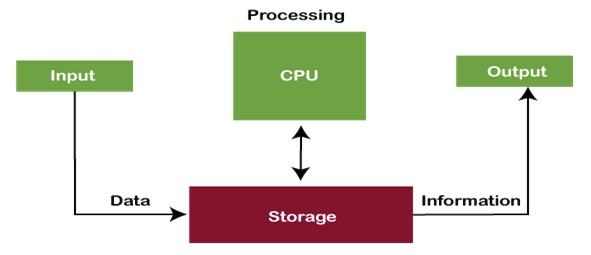
\includegraphics[width=1\textwidth]{Fig 1.jpg}
\caption{Computer Process}
\end{figure}
\section{History of computers}
Charles Babbage is considered to be the father of computer, for his invention
and the concept of Analytical Engine in 1837. The Analytical Engine contained an Arithmetic Logic Unit (ALU), basic flow control, and integrated memory; which led to the development of first general purpose computer concept.
\section{Generations of computer}
In the field of electronics and technology, generations of computer is a term that refers to the change that a computer goes through. Earlier, the term generation was used to differentiate between different hardware technologies. However, these days generation can be used to refer to both software and hardware; these together form the entire computer system.\\
\indent Growth in the computer industry is determined by the development in technology. Based on various stages of development, computers can be categorized into different generations.\\
\begin{wrapfigure}{r}{5cm}
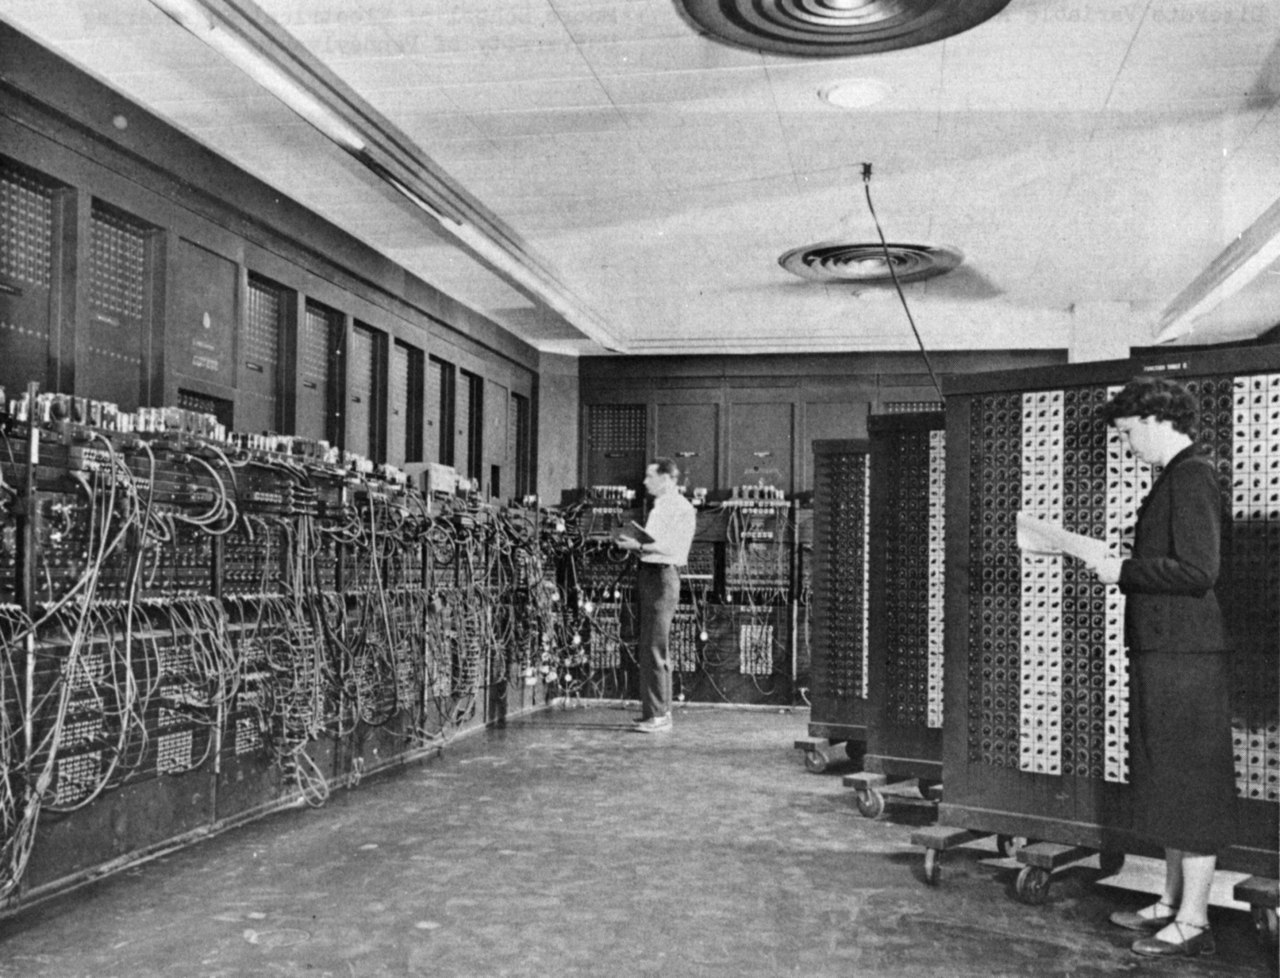
\includegraphics[width=5cm,height=5cm]{Fig 2.jpg}
\caption{A first generation computer}
\end{wrapfigure}
\subsection{First Generation}
\begin{itemize}
\item Period:1940-1956
\item Main Component Used:Vacuum Tubes
\item The first generation computers were big in size, consumed more power and was over heating.
\item Machine Language was used.
\item Examples of first generation computers are ENIAC, EDVAC and UNIVAC 1.
\end{itemize}
\subsection{Second Generation}
\begin{itemize}
    \item Period:1956-1964
    \item Main Component Used:Transistors
    \item The second generation computers were much smaller than the first one and also consumed less heat.
    \item First operating system was developed - Batch Processing and Multiprogramming Operating System.
    \item Punched cards were used.
    \item Machine language as well as Assembly language were used.  
    \item Examples of second generation computers are IBM 1401, IBM 1620, UNIVAC 1108.
\end{itemize}
\subsection{Third Generation}
\begin{itemize}
    \item Period:1964-1971
    \item Main Component Used:Integrated Circuits(IC)
    \item Computers were smaller, faster and more reliable.
    \item Consumed less power.
    \item High Level Languages were used.
    \item Examples of second generation computers are IBM 360 series, Honeywell 6000 series.
\end{itemize}
\subsection{Fourth Generation}
\begin{itemize}
    \item Period:1971-1980
    \item Main Component Used:Microprocessor
    \item These were smaller and faster computers than ever before.
    \item Portable Computers were introduced.
    \item This generation computers uses Very Large Scale Integrated Circuits
(VLSI).
    \item Microcomputer series such as IBM and APPLE were developed.
\end{itemize}
\subsection{Fifth Generation}
\begin{itemize}
    \item Period:1980-Present
    \item Parallel Processing.
    \item Super conductors.
    \item Computers size was drastically reduced.
    \item Can recognise Images and Graphics.
    \item Introduction of Artificial Intelligence and Expert Systems.
    \item Able to solve high complex problems including decision making and logical reasoning.
    \item This generation computers uses Ultra Large Scale Integrated Circuits
(ULSI).
\end{itemize}
\subsection{Sixth Generation}
\begin{itemize}
    \item Period:In Future
    \item Parallel and Distributed computing.
    \item Computers have become smarter, faster and smaller.
    \item Development of robotics.
    \item Can recognise Images and Graphics.
    \item Introduction of Artificial Intelligence and Expert Systems.
    \item Able to solve high complex problems including decision making and logical reasoning.  
\end{itemize}
\section{Introduction to computer}
Computer is a device for processing, storing, and displaying information.\par
Computer once meant a person who did computations, but now the term almost universally refers to automated electronic machinery. The first section of this article focuses on modern digital electronic computers and their design, constituent parts, and applications. The second section covers the history of computing.
\subsection{Computing basics}
The first computers were used primarily for numerical calculations. However, as any information can be numerically encoded, people soon realized that computers are capable of general-purpose information processing. Their capacity to handle large amounts of data has extended the range and accuracy of weather forecasting. Their speed has allowed them to make decisions about routing telephone connections through a network and to control mechanical systems such as automobiles, nuclear reactors, and robotic surgical tools. They are also cheap enough to be embedded in everyday appliances and to make clothes dryers and rice cookers “smart.” Computers have allowed us to pose and answer questions that could not be pursued before. These questions might be about DNA sequences in genes, patterns of activity in a consumer market, or all the uses of a word in texts that have been stored in a database. Increasingly, computers can also learn and adapt as they operate.\par
Computers also have limitations, some of which are theoretical. For example, there are not decidable propositions whose truth cannot be determined within a given set of rules, such as the logical structure of a computer. Because no universal algorithmic method can exist to identify such propositions, a computer asked to obtain the truth of such a proposition will (unless forcibly interrupted) continues indefinitely—a condition known as the “halting problem”. Other limitations reflect current technology. Human minds are skilled at recognizing spatial patterns—easily distinguishing among human faces, for instance—but this is a difficult task for computers, which must process information sequentially, rather than grasping details overall at a glance. Another problematic area for computers involves natural language interactions. Because so much common knowledge and contextual information is assumed in ordinary human communication, researchers have yet to solve the problem of providing relevant information to general-purpose natural language programs.

\subsection{Analog computers}
Analog computers use continuous physical magnitudes to represent quantitative information. At first they represented quantities with mechanical components, but after World War II voltages were used; by the 1960s digital computers had largely replaced them. Nonetheless, analog computers, and some hybrid digital-analog systems, continued in use through the 1960s in tasks such as aircraft and spaceflight simulation.\par
One advantage of analog computation is that it may be relatively simple to design and build an analog computer to solve a single problem. Another advantage is that analog computers can frequently represent and solve a problem in “real time”; that is, the computation proceeds at the same rate as the system being modeled by it. Their main disadvantages are that analog representations are limited in precision—typically a few decimal places but fewer in complex mechanised general-purpose devices are expensive and not easily programmed.

\subsection{Digital computers}
In contrast to analog computers, digital computers represent information in discrete form, generally as sequences of 0s and 1s (binary digits, or bits). The modern era of digital computers began in the late 1930s and early 1940s in the United States, Britain, and Germany. The first devices used switches operated by electromagnets (relays). Their programs were stored on punched paper tape or cards, and they had limited internal data storage.

\subsection{Mainframe computer}
During the 1950s and ’60s, Unisys (maker of the UNIVAC computer), International Business Machines Corporation (IBM), and other companies made large, expensive computers of increasing power. They were used by major corporations and government research laboratories, typically as the sole computer in the organization. In 1959 the IBM 1401 computer rented for 8,000 per month (early IBM machines were almost always leased rather than sold), and in 1964 the largest IBM S/360 computer cost several million dollars.\par
These computers came to be called mainframes, though the term did not become common until smaller computers were built. Mainframe computers were characterized by having (for their time) large storage capabilities, fast components, and powerful computational abilities. They were highly reliable, and, because they frequently served vital needs in an organization, they were sometimes designed with redundant components that let them survive partial failures. Because they were complex systems, they were operated by a staff of systems programmers, who alone had access to the computer. Other users submitted “batch jobs” to be run one at a time on the mainframe.\par
Such systems remain important today, though they are no longer the sole, or even primary, central computing resource of an organization, which will typically have hundreds or thousands of personal computers (PCs). Mainframes now provide high-capacity data storage for Internet servers, or, through time-sharing techniques, they allow hundreds or thousands of users to run programs simultaneously. Because of their current roles, these computers are now called servers rather than mainframes.
\subsection{Supercomputer}
The most powerful computers of the day have typically been called supercomputers. They have historically been very expensive and their use limited to high-priority computations for government-sponsored research, such as nuclear simulations and weather modeling. Today many of the computational techniques of early supercomputers are in common use in PCs. On the other hand, the design of costly, special-purpose processors for supercomputers has been supplanted by the use of large arrays of commodity processors (from several dozen to over 8,000) operating in parallel over a high-speed communications network.
\subsection{Minicomputer}
Although minicomputers date to the early 1950s, the term was introduced in the mid-1960s. Relatively small and inexpensive, minicomputers were typically used in a single department of an organization and often dedicated to one task or shared by a small group. Minicomputers generally had limited computational power, but they had excellent compatibility with various laboratory and industrial devices for collecting and inputting data.\par
One of the most important manufacturers of minicomputers was Digital Equipment Corporation (DEC) with its Programmed Data Processor (PDP). In 1960 DEC’s PDP-1 sold for 120,000 dollars. Five years later its PDP-8 cost 18,000 dollars and became the first widely used minicomputer, with more than 50,000 sold. The DEC PDP-11, introduced in 1970, came in a variety of models, small and cheap enough to control a single manufacturing process and large enough for shared use in university computer centers; more than 650,000 were sold. However, the microcomputer overtook this market in the 1980s.
\subsection{Microcomputer}
A microcomputer is a small computer built around a microprocessor integrated circuit, or chip. Whereas the early minicomputers replaced vacuum tubes with discrete transistors, microcomputers (and later minicomputers as well) used microprocessors that integrated thousands or millions of transistors on a single chip. In 1971 the Intel Corporation produced the first microprocessor, the Intel 4004, which was powerful enough to function as a computer although it was produced for use in a Japanese-made calculator. In 1975 the first personal computer, the Altair, used a successor chip, the Intel 8080 microprocessor. Like minicomputers, early microcomputers had relatively limited storage and data-handling capabilities, but these have grown as storage technology has improved alongside processing power.
\section{Hardware and Software}
\subsection{Hardware}
The physical elements of a computer, its hardware, are generally divided into the central processing unit (CPU), main memory (or random-access memory, RAM), and peripherals. The last class encompasses all sorts of input and output (I/O) devices: keyboard, display monitor, printer, disk drives, network connections, scanners, and more.\par
The CPU and RAM are integrated circuits (ICs)—small silicon wafers, or chips, that contain thousands or millions of transistors that function as electrical switches. In 1965 Gordon Moore, one of the founders of Intel, stated what has become known as Moore’s law: the number of transistors on a chip doubles about every 18 months. Moore suggested that financial constraints would soon cause his law to break down, but it has been remarkably accurate for far longer than he first envisioned. It now appears that technical constraints may finally invalidate Moore’s law, since sometime between 2010 and 2020 transistors would have to consist of only a few atoms each, at which point the laws of quantum physics imply that they would cease to function reliably. 
\subsection{Software}
Software are instructions that tell a computer what to do. Software comprises the entire set of programs, procedures, and routines associated with the operation of a computer system. The term was coined to differentiate these instructions from hardware—i.e., the physical components of a computer system. A set of instructions that directs a computer’s hardware to perform a task is called a program, or software program.\par
The two main types of software are system software and application software. System software controls a computer’s internal functioning, chiefly through an operating system, and also controls such peripherals as monitors, printers, and storage devices. Application software, by contrast, directs the computer to execute commands given by the user and may be said to include any program that processes data for a user. Application software thus includes word processors, spreadsheets, database management, inventory and payroll programs, and many other “applications.” A third software category is that of network software, which coordinates communication between the computers linked in a network.\par
Software is typically stored on an external long-term memory device, such as a hard drive or magnetic diskette. When the program is in use, the computer reads it from the storage device and temporarily places the instructions in random access memory (RAM). The process of storing and then performing the instructions is called “running,” or “executing,” a program. By contrast, software programs and procedures that are permanently stored in a computer’s memory using a read-only (ROM) technology are called firmware, or “hard software.”
\section{Operating Systems}
\subsection{MS-DOS}
MS-DOS which is short for Microsoft Disk Operating System is a non-graphical command line operating system developed for IBM compatible computers with x86 microprocessor. The operating system used a command line interface for the user to input commands to navigate open and manipulate files on their computer.
\begin{figure}[H]
\centering 
\includegraphics[scale=1]{Fig 3.jpg}
\caption{The MS-Dos Logo}
\end{figure}
Features:
\begin{itemize}
    \item It is a single user operating system meaning only one user can operate at a time.
    \item It is a light weight operating system allowing users to have direct access to the BIOS and its underlying hardware.
    \item Loads data and programs from external sources and bring them into the internal memory so they can be used on the computer.
    \item Enables the computer to perform input and output operations such as taking commands from keyboard, printing information on the screen.
    \item It is very helpful in making file management like creating, editing, deleting files, etc.
    \item It also controls and manages other external devices such as the printer, keyboard or external hard drive using various drive utilities.
\end{itemize}
Drawbacks:
\begin{itemize}
    \item It does not allow multiple users to operate on the system.
    \item It does not support graphical interface hence mouse cannot be used to operate it.
    \item It does not support multiprogramming meaning it can only have one process in the ram.
    \item It lacked memory protection which meant no security, and less stability.
    \item It has difficulty in memory access when addressing more than 640 MB of RAM.
\end{itemize}
\subsection{Windows Operating System}
\begin{wrapfigure}{r}{5cm}
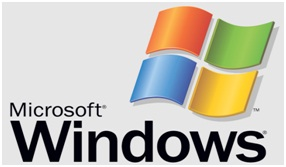
\includegraphics[width=5cm]{Fig 4.jpg}
\caption{The Windows Logo}
\end{wrapfigure}
Windows is an operating system designed by Microsoft to be used on a standard x86 Intel and AMD processors. It provides an interface, known as a graphical user interface (GUI) which eliminates the need to memorize commands for the command line by using a mouse to navigate through menus, dialog boxes, buttons, tabs, and icons. The operating system was named windows since the programs are displayed in the shape of a square. This Windows operating system has been designed for both a novice user just using at home as well as for professionals who are into development.\\
\newline
Features:
\begin{itemize}
    \item It is designed to run on any standard x86 Intel and AMD hence most of the hardware vendors make drivers for windows like Dell, HP, etc.
\item It supports enhanced performance by utilizing multi-core processors.
\item It comes preloaded with many productivity tools which helps to complete all types of everyday tasks on your computer.
\item Windows has a very large user base so there is a much larger selection of available software programs, utilities.
\item Windows is backward compatible meaning old programs can run on newer versions.
\item Hardware is automatically detected eliminating need of manually installing any device drivers.
\end{itemize}
Drawbacks:
\begin{itemize}
    \item Windows can be expensive since the OS is paid license and majority of its applications are paid products.
\item Windows has high computer resource requirement like it should have high ram capacity, a lot of hard drive space and good graphics card.
\item Windows slows and hangs up if the user loads up many programs at the same time.
\item Windows includes network sharing that can be useful if user has a network with many PCs.
\item Windows is vulnerable to virus attacks since it has a huge user base and users have to update OS to keep up-to-date with security patches.
\end{itemize}
\subsection{LINUX Operating System}
The Linux OS is an open source operating system project that is a freely distributed, cross-platform operating system developed based on UNIX. This operating system is developed by Linus Torvalds. The name Linux comes from the Linux kernel. It is basically the system software on a computer that allows apps and users to perform some specific task on the computer.\par
\begin{wrapfigure}{r}{5cm}

\includegraphics[width=5cm]{Fig 5.jpg}
\caption{The Linux Logo}
\end{wrapfigure}
The development of Linux operating system pioneered the open source development and became the symbol of software collaboration.\\
\newline
Features:
\begin{itemize}
\item Linux is free can be downloaded from the Internet or redistribute it under GNU licenses and has the best community support.
\item Linux OS is easily portable which means it can be installed on various types of devices like mobile, tablet computers.
\item It is a multi-user, multitasking operating system.
\item BASH is the Linux interpreter program which can be used to execute commands.
\item Linux provides multiple levels of file structures i.e. hierarchical structure in which all the files required by the system and those that are created by the user are arranged.
\item Linux provides user security using authentication features and also threat detection and solution is very fast because Linux is mainly community driven.
\end{itemize}	
Drawbacks:
\begin{itemize}
\item There’s no standard edition of Linux hence confusing for users and also becoming familiar with the Linux may be a problem for new users.
\item More difficult to find applications to support user needs since Linux does not dominate the market.
\item Since some applications are developed specifically for Windows and Mac, those might not be compatible with Linux and sometimes users might not have much of a choice to choose between different applications like in Windows or Mac since most apps are developed for operating systems that have a huge user base.
\item Some hardware may not be incompatible with Linux since it has patchier support for drivers which may result in malfunction.
\item There are plenty of forums to resolve Linux issues, but it may not always match the user’s own level of technical understanding.
\end{itemize}
\subsection{Solaris Operating System}
\begin{wrapfigure}{r}{5cm}

\includegraphics[width=5cm,height=3cm]{Fig 6.jpg}
\caption{The Solaris Logo}
\end{wrapfigure}
Solaris or SunOS is the name of the Sun Company’s UNIX variant operating system that was originally developed for its family of Scalable Processor Architecture-based processors (SPARC) as well as for Intel-based processors. The UNIX workstation market had been largely dominated by this operating system during its time. As the Internet grew Sun’s Solaris systems became the most widely installed servers for Web sites. Oracle purchased Sun and later renamed to Oracle Solaris.
\newline
Features:
\begin{itemize}
\item Solaris is known for its scalability. It can handle a large workload and still delivers indisputable performance advantages for database, Web, and Java technology-based services.
\item Solaris systems were known to their availability meaning that these operating systems hardly crashes at anytime and because of its internet networking oriented design and broad scope of features it makes the job of adding new features or fixing any problems easy.
\item It is built for network computing as it provides optimized network stack and support for advanced network computing protocols that delivers high-performance networking to most applications.
\item Solaris has advanced, unique security capabilities which includes some of the world’s most advanced security features, such as user rights management, cryptographic Framework and secure by default networking that allows users to safely deliver new solutions.
\item Provides tools to enable seamless interoperability, test new software and efficiently consolidate application workloads.
\end{itemize}
Drawbacks:
\begin{itemize}
\item Solaris is quite expensive since it’s an enterprise operating system. Also, Solaris doesn’t provide updates for free.
\item Solaris lacks a good graphical user interface support and is not user friendly.
\item Hardware support is not nearly as good as many other operating systems.
\item Performance would degrade considerably since Solaris cannot make use of different hardware that efficiently.
\item Solaris sometimes becomes unstable and crashes due to total consumption of CPU and memory.
\end{itemize}
\subsection{Symbian Operating System}
Symbian OS was the most widely-used smartphone operating system in the world based on ARM architecture, until it was discontinued in 2014. It was developed by Symbiant Ltd, which was a partnership among PDA devices and smartphone manufacturers like Psion, Motorola, Ericsson, and Nokia. The Symbian Operating System was developed of two sub system where the first is the microkernel-based operating system with its associated libraries, and the other being interface of the OS with which the user interacts. It was explicitly developed for smartphones and hand held digital devices since this operating system consumes very low power, battery-based devices and also for ROM-based systems.\\
\begin{wrapfigure}{r}{5cm}
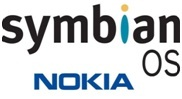
\includegraphics[width=5cm]{Fig 7.jpg}
\caption{The Symbian Logo}
\end{wrapfigure}
Features:
\begin{itemize}
    \item Its kernel known as EKA2 features preemptive multithreading, scheduling, memory management system and device drivers.
\item Allows third party software to enhance the platform for better performance of the operating system.
\item Symbian Interface is easy to use and very user friendly.
\item Applications for Symbian are normally written in C++ or Symbian C++ using Symbian Software Development Kit (SDK).
\item Symbian can also run applications written in Python, Java ME, Flash Lite, Ruby and .NET.
\item Connectivity is lot easier and faster.
\item Symbian OS has good efficiency and stability.
\end{itemize}
Drawbacks:
\begin{itemize}
    \item Responsiveness is not smooth and sensitive as other operating systems.
\item The Symbian OS is very vulnerable and can be easily affected by a Virus.
\item Lack of virtual memory.
\end{itemize}
\subsection{Android OS}
Android is a Google’s Linux based operating system it is designed primarily for touch screen mobile devices such as smart phones and tablet computers. The hardware which can be used to support android is based on three architectures namely ARM, Intel and MIPS design lets users manipulate the mobile devices intuitively, with finger movements that mirror common motions, such as pinching, swiping, and tapping making these applications comfortable for the users.\\
\begin{wrapfigure}{r}{4cm}

\includegraphics[width=4cm]{Fig 8.jpg}
\caption{Android Logo}
\end{wrapfigure}
Features:
\begin{itemize}
    \item The android operating system is an open source operating system means that it’s free and any one can use it.
\item Android offers optimized 2D and 3D graphics, multimedia, GSM connectivity, multi-tasking.
\item Android OS is known for its friendly user interface and exceptional customizable according to the user’s taste.
\item Huge choice of applications for its users since Playstore offers over one million apps.
\item Software developers who want to create applications for the Android OS can download the Android Software Development Kit (SDK) to easily develop apps for android.
\item Android would consume very little power but deliver extreme performance since its hardware is based on ARM architecture.
\end{itemize}
Drawbacks:
\begin{itemize}
    \item The design and coding of intuitive modern user experiences and interfaces poses a difficulty because of its dependency on Java.
\item Most apps tend to run in the background even when closed by the user draining the battery.
\item Performance is bound to take a hit as multiple programs run simultaneously in the background at any given time.
\item Android phones overheat especially when indulged in hardcore productivity tasks or heavy graphics.
\item Apps have lower security profiles and make users more susceptible to data breaches.
\end{itemize}
\subsection{iOS Mobile Operating System}
iOS which is short for iPhone OS is a mobile operating system created and developed by Apple Inc. exclusively for its hardware like A12 Bionic chip that presently powers many of its mobile devices, including the iPhone, iPad, and iPod. The iOS user interface is based upon using multi-touch gestures such as swipe, tap, pinch, and reverse pinch. The purpose of these finger actions is to provide the user with fast responsive inputs given from multiple fingers to the multi-touch capacitive screen display.
\begin{wrapfigure}{r}{5cm}

\includegraphics[width=5cm,height=2cm]{Fig 9.jpg}
\caption{The iOS Logo}
\end{wrapfigure}
Features:
\begin{itemize}
\item It is written in C, C++, Objective-C and Swift and is based on the Macintosh OS X.
\item Has excellent and intuitive user interface and very fluid response.
\item Performance of iOS is unbeatable.
\item iOS comes with a lot of default apps, including an email client, web browser, media player and the phone app.
\item Availability of higher quality apps which can be downloaded from the Appstore.
\item Apple has provided its own iOS software development kit (SDK) for the developers to create applications for Apple mobile devices.
\item iOS is much safer than other mobile operating systems and has fewer security breaches as well.
\item Provides regular updates and 
\end{itemize}
Drawbacks:
\begin{itemize}
    \item The OS is closed source instead of open source hence beta testing taking a lot of time since its only available to limited developers.
\item The amount of memory space the iOS applications occupy is very large when compared with other mobile platforms.
\item Lack of customization compared to other operating systems.
\item Doesn’t allow third party installations.
\item Having intense graphics and animations consumes more power and causes battery drains.
\item iOS is resource intensive operating system due to which older devices struggle to run it.
\end{itemize}
\section{Suitable Operating Systems}
These are explained as following below.
\subsection{Database and Web Server Management}
The best suitable operating system for database and web server management is SOLARIS, is Unix Operating system, which itself is designed for enterprise web servers where robust applications and database is deployed where throughput is very high and needs the server 24×7 up and less down time.
\subsection{Cluster Computing}
Clustering is a technique where multiple computers, storage devices and redundant interconnections are used to create a single highly available system. Each computer in it is a node. The best preferred operating system for cluster computing is LINUX which is a UNIX based open source freely distributed operating system which offers many robust network features.
\subsection{Productivity and Daily Tasks}
The best suitable operating system for productivity is WINDOWS because it is intuitive, cohesive, functional and very user friendly. Windows offers best selection of software and can run on widest variety of hardware that the user has.
\newpage
\part{Computer components}
Computer's various component:
\begin{itemize}
\item A Central Processing Unit (CPU)
\item Memory RAM
\item ROM
\item ALU (arithmetic logic unit)
\item Display devices
\item Hardcopy devices
\item Input devices
\end{itemize}
\section{Central processing unit}
Central processing unit (CPU), principal part of any digital computer system, generally composed of the main memory, control unit, and arithmetic-logic unit. It constitutes the physical heart of the entire computer system; to it is linked various peripheral equipment, including input/output devices and auxiliary storage units. In modern computers, the CPU is contained on an integrated circuit chip called a microprocessor.\par
The control unit of the central processing unit regulates and integrates the operations of the computer. It selects and retrieves instructions from the main memory in proper sequence and interprets them so as to activate the other functional elements of the system at the appropriate moment to perform their respective operations. All input data are transferred via the main memory to the arithmetic-logic unit for processing, which involves the four basic arithmetic functions (i.e., addition, subtraction, multiplication, and division) and certain logic operations such as the comparing of data and the selection of the desired problem-solving procedure or a viable alternative based on predetermined decision criteria.
\section{Memory RAM}
Which stands for Random Access Memory, is a hardware device generally located on the motherboard of a computer and acts as an internal memory of the CPU? It allows CPU store data, program, and program results when you switch on the computer. It is the read and writes memory of a computer, which means the information can be written to it as well as read from it.\par
RAM is a volatile memory, which means it does not store data or instructions permanently. When you switch on the computer the data and instructions from the hard disk are stored in the RAM, e.g., when the computer is rebooted, and when you open a program, the operating system (OS), and the program are loaded into RAM, generally from an HDD or SSD. CPU utilizes this data to perform the required tasks. As soon as you shut down the computer, the RAM loses the data. So, the data remains in the RAM as long as the computer is on and lost when the computer is turned off. The benefit of loading data into RAM is that reading data from the RAM is much faster than reading from the hard drive.\par
In simple words, we can say that RAM is like a person’s short term memory, and hard drive storage is like a person's long term memory. Short term memory remembers the things for a short duration, whereas long term memory remembers for a long duration. Short term memory can be refreshed with information stored in the brain’s long term memory. A computer also works like this; when the RAM fills up, the processor goes to the hard disk to overlay the old data in Ram with new data. It is like a reusable scratch paper on which you can write notes, numbers, etc., with a pencil. If you run out of space on the paper, you may erase what you no longer need; RAM also behaves like this, the unnecessary data on the RAM is deleted when it fills up, and it is replaced with new data from the hard disk which is required for the current operations.\par
RAM comes in the form of a chip that is individually mounted on the motherboard or in the form of several chips on a small board connected to the motherboard. It is the main memory of a computer. It is faster to write to and read from as compared to other memories such as a hard disk drive (HDD), solid-state drive (SSD), optical drive, etc.\par
\begin{figure}[H]
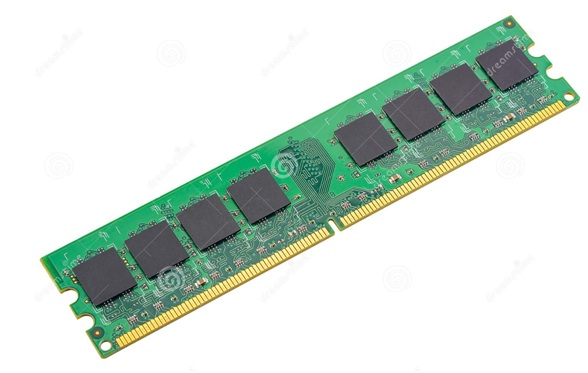
\includegraphics[width=1\textwidth]{Fig 10.jpg}
\caption{RAM Module}
\end{figure}
A computer's performance mainly depends on the size or storage capacity of the RAM. If it does not have sufficient RAM (random access memory) to run the OS and software programs, it will result in slower performance. So, the more RAM a computer has, the faster it will work. Information stored in RAM is accessed randomly, not in a sequence as on a CD or hard drive. So, its access time is much faster.
\section{Memory ROM}
Read-only memory (ROM) is a class of storage medium used in computers and other electronic devices. Data stored in ROM can only be modified slowly, with difficulty, or not at all, so it is mainly used to distribute firmware (software that is very closely tied to specific hardware and unlikely to need frequent updates)\par
Read-only memory (ROM) is a type of storage medium that permanently stores data on personal computers (PCs) and other electronic devices.\par
It contains the programming needed to start a PC, which is essential for boot-up; it performs major input/output tasks and holds programs or software instructions.\par 
Because ROM is read-only, it cannot be changed; it is permanent and non-volatile, meaning it also holds its memory even when power is removed.\par
In a typical modern computer, there are numerous ROM chips located on the motherboard and a few on expansion boards. The chips are essential for the basic input/output system (BIOS), boot up, reading and writing to peripheral devices, basic data management and the software for basic processes for certain utilities.\begin{figure}[H]
\centering 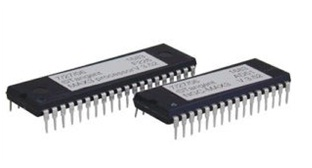
\includegraphics[scale=1]{Fig 11.jpg}
\caption{An old age ROM device}
\end{figure}
\section{Hardcopy devices}
Hard copy devices are those that give the output in the tangible form. Printers and Plotters are two common hard copy devices. Impact printers are those printers in which there is a direct contact between the printing head and the paper on which the print is produced.\par
A hard copy (or "hardcopy") is a printed copy of information from a computer. Sometimes referred to as a printout, a hard copy is so-called because it exists as a physical object. The same information, viewed on a computer display or sent as an e-mail attachment, is sometimes referred to as a soft copy.\par 
Alternatively referred to as a paper copy, a hard copy is any information that is printed on paper. Hard copies allow data to be read without the need of a computer and are often required when someone needs to sign a document.\\
How is a hard copy produced by a computer?\par
A hard copy can be created using a printer (e.g., dot matrix printer, inkjet printer, laser printer, etc.) and a typewriter.
The quality of the hard copy is determined by DPI (dots per inch) of the printer being used. Typically, a laser printer has the highest quality.\\
Why would someone need to make a hard copy?\par
As more and more people move to digital and paperless solutions, there are not many reasons to make a hard copy. However, hard copies still find some uses which we've listed below.
\begin{enumerate}
    \item They are useful when a paper needs to be signed.
\item They are needed for someone who doesn't have access to a computer or digital device.
\item They are needed for reports for school.
\item They are needed when a print out for legal filing or taxes that requires a hard copy.
\item They are needed for copies of receipts, proof of purchase, or completed service.
\end{enumerate}
\section{Difference between Hard Copy and Soft Copy}
\subsection{Hard Copy}
Hard copy refers to the digital document file which is printed on paper or other material like transparency. In hard copy the output is printed on the paper and sometimes it is referred as permanent copy. We can touch the hard copy. We can say it is a physical copy.For example- Book, Notebook, printed document files, etc. 
\subsection{Soft Copy}
Soft copy refers to the digital document file or electronic version of a document that is not printed on paper. In soft copy the output is present in the USB drives and computers etc and sometimes it is referred as temporary copy. We cannot touch the soft copy. We can say it is a virtual copy. For example- EBooks, PDF notes, scanned notes etc.
\section{Arithmetic and Logic unit}
\begin{figure}[H]
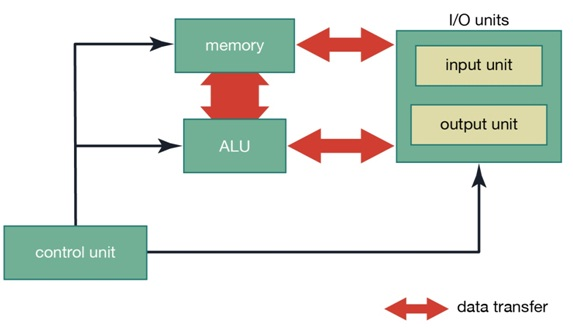
\includegraphics[width=1\textwidth]{Fig 12.jpg}
\caption{Computer's data transfer flowchart}
\end{figure}
In the computer system, ALU is a main component of the central processing unit, which stands for arithmetic logic unit and performs arithmetic and logic operations. It is also known as an integer unit (IU) that is an integrated circuit within a CPU or GPU, which is the last component to perform calculations in the processor. It has the ability to perform all processes related to arithmetic and logic operations such as addition, subtraction, and shifting operations, including Boolean comparisons (XOR, OR, AND, and NOT operations). Also, binary numbers can accomplish mathematical and bitwise operations. The arithmetic logic unit is split into AU (arithmetic unit) and LU (logic unit). The operands and code used by the ALU tell it which operations have to perform according to input data. When the ALU completes the processing of input, the information is sent to the computer's memory.  
Except performing calculations related to addition and subtraction, ALUs handle the multiplication of two integers as they are designed to execute integer calculations; hence, its result is also an integer. However, division operations commonly may not be performed by ALU as division operations may produce a result in a floating-point number. Instead, the floating-point unit (FPU) usually handles the division operations; other non-integer calculations can also be performed by FPU.\par
Additionally, engineers can design the ALU to perform any type of operation. However, ALU becomes more costly as the operations become more complex because ALU destroys more heat and takes up more space in the CPU. This is the reason to make powerful ALU by engineers, which provides the surety that the CPU is fast and powerful as well.\par
The calculations needed by the CPU are handled by the arithmetic logic unit (ALU); most of the operations among them are logical in nature. If the CPU is made more powerful, which is made on the basis of the ALU is designed. Then it creates more heat and takes more power or energy. Therefore, it must be moderation between how complex and powerful ALU is and not be more costly. This is the main reason the faster CPUs are more costly; hence, they take much power and destroy more heat. Arithmetic and logic operations are the main operations that are performed by the ALU; it also performs bit-shifting operations.
\section{I/O devices}
\subsection{Input Devices}
\begin{figure}[H]
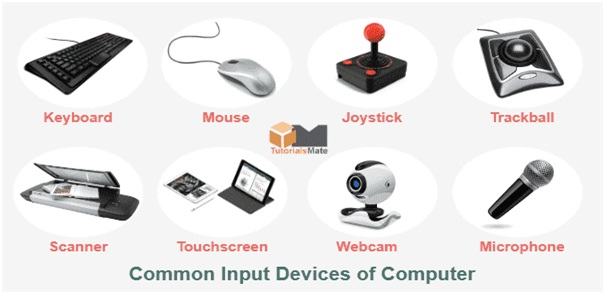
\includegraphics[width=1\textwidth]{Fig 13.jpg}
\caption{Input Devices}
\end{figure}
An input device is essentially a piece of hardware that sends data to a computer. Most input devices either interact with control of the computer in some way. The most common input devices are the mouse and the keyboard, but there are many others.\par
The key distinction between an input device and an output device is that the former sends data to the computer, whereas the latter receives data from the computer. Input and output devices that provide computers with additional functionality are also called peripheral or auxiliary devices.\par
The most commonly used or primary input devices on a computer are the keyboard and mouse. However, there are other devices that input data into a computer.  
\noindent What are the input devices of my computer?\par
Every computer comes with a keyboard and a mouse (touchpad with laptop), which are considered input devices. As far as other input devices, it depends on what was included with your computer and what's connected to the computer. The best method of determining all of the input devices your computer has is to go through the list above.\\
What does an input device send to a computer?\par
An input device sends (inputs) to a computer depends on the device. Additionally, all input devices send data from the device over a cable or wireless transmission to the computer. For example, as you move a computer mouse, the data sent to the computer is the X-Y axis movements used to display the mouse cursor on the screen. You can see a live example of this on our x-axis definition.\\
Why does a computer need an input device?\par
Today, input devices are important because they are what allow you to interact with and add new information to a computer. For example, if a computer had no input devices, it could run by itself but there would be no way to change its settings, fix errors, or other various user interactions. Also, if you wanted to add new information to the computer (e.g., text, command, document, picture, etc.), you wouldn't be able to do so without an input device.\\
Input devices for physically challenged users:\\
In addition to the list mentioned above, other specially designed input devices are designed for the physically challenged. Below is a list of examples of these devices.
\begin{itemize}
\item Eye-tracking - A specialized camera to track a user's eye to perform actions or move a mouse pointer.
\item Foot mouse - Mouse pointer controlled using pedals with your feet.
\item Gesture recognition - Specialized device to detect different gestures, including facial expressions, reading lips, and sign language.
\item Head-mounted pointer - A pointer can be mounted to a hat or band to track and control the mouse pointer.
\item Joystick - A joystick next to the computer or on a wheelchair to control a mouse pointer. It's possible these joysticks could be operated using your chin, lips, or tongue for people with no head movement.
\item Voice recognition - Using your voice to control computer functions and typing on a computer.
\end{itemize}
\subsection{Output Device}
The output device displays the result of the processing of raw data that is entered in the computer through an input device. There are a number of output devices that display output in different ways such as text, images, hard copies, and audio or video.\\
Following are some of the important output devices used in a computer.
\begin{itemize}
    \item Monitors
\item Graphic Plotters
\item Printers
\end{itemize}
\section{Display devices}
The display devices are output devices to display the information in visual form by means of various types of display systems. In digital instruments, the output device of the instrument indicates the value of measured quantity using the digital display device. This digital display device may receive the digital information in any form but it converts the information in decimal form. The digital display device indicates the value in decimal digits directly. LEDs are most commonly used in digital displays for displaying alphanumeric characters. The LEDs have advantages such as low voltage, long life, high reliability, low cost, fast switching characteristics, etc.\\
Classification of Display\\
The most commonly used display devices are CRT (Cathode Ray Tube), LED (Light Emitting Diode) and LCD (Liquid Crystal Display), etc. In the digital electronics field, the commonly used display devices are given as follows:\\
Types of display devices –
\begin{enumerate}
    \item Light Emitting Diode (LED)
\item Liquid Crystal Display (LCD)
\item Nixie Tube or Cold Cathode Displays
\item Incandescent Displays
\item Fluorescent Displays
\item Liquid Vapor Based Display
\item Segmented Gas Discharge Displays	
\end{enumerate}
    
Monitors, commonly called as Visual Display Unit (VDU), are the main output device of a computer. It forms images from tiny dots, called pixels that are arranged in a rectangular form. The sharpness of the image depends upon the number of pixels. \\
There are two kinds of viewing screen used for monitors.
\begin{itemize}
    \item Cathode-Ray Tube (CRT)
\item Flat-Panel Display
\end{itemize}
 \subsection{Cathode-Ray Tube (CRT) Monitor}
 The CRT display is made up of small picture elements called pixels. The smaller the pixels, the better the image clarity or resolution. It takes more than one illuminated pixel to form a whole character, such as the letter ‘e’ in the word help.\\
 A finite number of characters can be displayed on a screen at once. The screen can be divided into a series of character boxes - fixed location on the screen where a standard character can be placed. Most screens are capable of displaying 80 characters of data horizontally and 25 lines vertically. \\
There are some disadvantages of CRT – 
\begin{itemize}
    \item Large in Size  
\item High power consumption
\end{itemize}
\subsection{Flat-Panel Display Monitor} 
The flat-panel display refers to a class of video devices that have reduced volume, weight and power requirement in comparison to the CRT. You can hang them on walls or wear them on your wrists. Current uses of flat-panel displays include calculators, video games, monitors, laptop computer, and graphics display.
\begin{figure}[H]
\centering 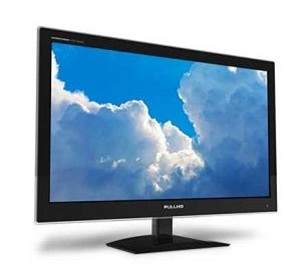
\includegraphics[scale=1]{Fig 14.jpg}
\caption{Flat Panel Display}
\end{figure}
\noindent \textbf{The flat-panel display is divided into two categories –}\\
Emissive Displays: Emissive displays are devices that convert electrical energy into light. For example, plasma panel and LED (Light-Emitting Diodes).\\  
Non-Emissive Displays: Non-emissive displays use optical effects to convert sunlight or light from some other source into graphics patterns. For example, LCD (Liquid Crystal Device).

\section{Printers}  Printer is an output device, which is used to print information on paper. \\
There are two types of printers:  
\begin{itemize}
    \item Impact Printers
\item Non-Impact Printers
\end{itemize}
\subsection{Impact Printers}
Impact printers print the characters by striking them on the ribbon, which is then pressed on the paper. \\
Characteristics of Impact Printers are the following:  
\begin{itemize}
    \item Very low consumable costs
\item Very noisy
\item Useful for bulk printing due to low cost
\item There is physical contact with the paper to produce an image 
\end{itemize}
These printers are of two types:
\begin{itemize}
    \item Character printers
\item Line printers
\end{itemize}
Character Printers \\
Character printers are the printers which print one character at a time. \\
These are further divided into two types: 
\begin{itemize}
    \item Dot Matrix Printer(DMP)
\item Daisy Wheel
\end{itemize}
Dot Matrix Printer \\
In the market, one of the most popular printers is Dot Matrix Printer. These printers are popular because of their ease of printing and economical price. Each character printed is in the form of pattern of dots and head consists of a Matrix of Pins of size (5*7, 7*9, 9*7 or 9*9) which comes out to form a character which is why it is called Dot Matrix Printer.
\begin{figure}[H]
\centering 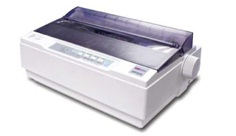
\includegraphics[scale=1]{Fig 15.jpg}
\caption{Dot Matrix Printer}
\end{figure}
Advantages  
\begin{itemize}
    \item Inexpensive  
\item Widely Used
\item Other language characters can be printed
\end{itemize}
Disadvantages  
\begin{itemize}
    \item Slow Speed
\item Poor Quality
\end{itemize}
Daisy Wheel \\
Head is lying on a wheel and pins corresponding to characters are like petals of Daisy (flower) which is why it is called Daisy Wheel Printer. These printers are generally used for word-processing in offices that require a few letters to be sent here and there with very nice quality.
\begin{figure}[H]
\centering 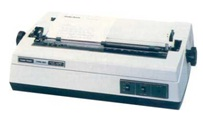
\includegraphics[scale=1]{Fig 16.jpg}
\caption{Daisy Wheel Printer}
\end{figure}
\noindent Advantages 
\begin{itemize}
    \item More reliable than DMP
\item Better quality
\item Fonts of character can be easily changed
\end{itemize}
Disadvantages  
\begin{itemize}
    \item Slower than DMP
\item Noisy
\item More expensive than DMP
\end{itemize}
Line Printers \\
Line printers are the printers which print one line at a time.\\
These are of two types:  
\begin{itemize}
    \item Drum Printer
\item Chain Printer
\end{itemize}
Drum Printer\par 
This printer is like a drum in shape hence it is called drum printer. The surface of the drum is divided into a number of tracks. Total tracks are equal to the size of the paper, i.e. for a paper width of 132 characters, drum will have 132 tracks. A character set is embossed on the track. Different character sets available in the market are 48 character set, 64 and 96 characters set. One rotation of drum prints one line. Drum printers are fast in speed and can print 300 to 2000 lines per minute. 
\begin{figure}[H]
\centering 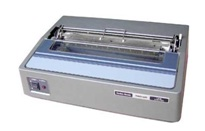
\includegraphics[scale=1]{Fig 17.jpg}
\caption{Drum Printer}
\end{figure}
\noindent Advantages  
\begin{itemize}
    \item Very high speed
\end{itemize}
Disadvantages  
\begin{itemize}
    \item Very expensive
\item Characters fonts cannot be changed
\end{itemize}
Chain Printer\par 
In this printer, a chain of character sets is used; hence it is called Chain Printer. A standard character set may have 48, 64, or 96 characters. \\
Advantages:
\begin{itemize}
    \item Character fonts can easily be changed.
\item Different languages can be used with the same printer.
\end{itemize}
Disadvantages:
\begin{itemize}
    \item Noisy
\end{itemize}
\subsection{Non-impact Printers} 
Non-impact printers print the characters without using the ribbon. These printers print a complete page at a time, thus they are also called as Page Printers. \\
These printers are of two types:  
\begin{itemize}
    \item Laser Printers  
\item Inkjet Printers
\end{itemize}
Characteristics of Non-impact Printers  
\begin{itemize}
    \item Faster than impact printers
\item They are not noisy
\item High quality
\item Supports many fonts and different character size
\end{itemize}
Laser Printers: \par
These are non-impact page printers. They use laser lights to produce the dots needed to form the characters to be printed on a page.
\begin{figure}[H]
\centering 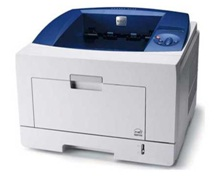
\includegraphics[scale=1]{Fig 18.jpg}
\caption{Laser Printer}
\end{figure}
\noindent Advantages:
\begin{itemize}
    \item Very high speed  
\item Very high quality output
\item Good graphics quality
\item Supports many fonts and different character size
\end{itemize}

Disadvantages:
\begin{itemize}
    \item Expensive  
\item Cannot be used to produce multiple copies of a document in a single printing
\end{itemize}
Inkjet Printers:\par
Inkjet printers are non-impact character printers based on a relatively new technology. They print characters by spraying small drops of ink onto paper. Inkjet printers produce high quality output with presentable features.\par
They make less noise because no hammering is done and these have many styles of printing modes available. Color printing is also possible. Some models of Inkjet printers can produce multiple copies of printing also.
\begin{figure}[H]
\centering 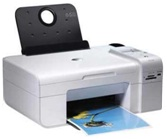
\includegraphics[scale=1]{Fig 19.jpg}
\caption{Inkjet Printer}
\end{figure}
\noindent Advantages:
\begin{itemize}
    \item High quality printing  
\item More reliable
\end{itemize}
Disadvantages:
\begin{itemize}
    \item Expensive as the cost per page is high  
\item Slow as compared to laser printer
\end{itemize}
\newpage
\part{Computer application in Radiology}
Computers play a major role in bridging the gap between image generation and patient care by providing enhanced images that better meet the needs of referring physicians. Spiral computed tomography allows generation of three-dimensional images that are not affected by motion artifact.\par
Currently, technologic computer advances play an important role in three clinical areas: orthopedic applications, oncologic applications, and prosthetic design. Three-dimensional imaging is especially valuable in fracture assessment because it allows exploration of image data to define the location of fracture fragments, the integrity of the joint space, and any possible displacement.\\
Medical image classification and Application\par
The medical imaging of medical research and clinical diagnosis are varied. It mainly divided into two categories, structural image and functional imaging technology. The former is mainly used to obtain the anatomical structure of the human body image, the clear picture of the human body structure and detailed pathological information can provides the reliable means for clinical medicine and medical science research. CT and MRI is a representative of this kind of structure.
Ultrasonic image application\par
Ultrasonic image is one of the four major imaging methods in the current imaging diagnosis. It uses the interaction between ultrasound and biology as imaging basis. It has no ionizing radiation, non radioactive, without contraindication, examination time is short, equipment low price advantage, particularly suitable for inspection and diagnosis of soft tissue and organ motion
\section{ADC (Analog to Digital Converter)} 
\begin{figure}[H]
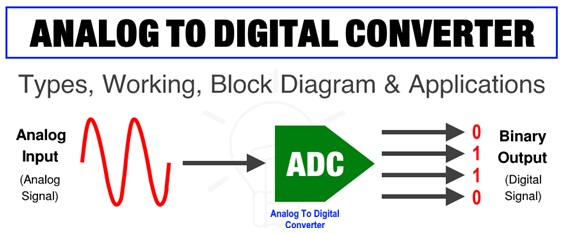
\includegraphics[width=1\textwidth]{Fig 20.jpg}
\caption{Analog to Digital Converter}
\end{figure}
Almost every environmental measurable parameter is in analog form like temperature, sound, pressure, light, etc. Consider a temperature monitoring system wherein acquiring, analyzing, and processing temperature data from sensors is not possible with digital computers and processors. Therefore, this system needs an intermediate device to convert the analog temperature data into digital data in order to communicate with digital processors like microcontrollers and microprocessors.\par 
A converter that is used to change the analog signal to digital is known as an analog to digital converter or ADC converter. This converter is one kind of integrated circuit or IC that converts the signal directly from continuous form to discrete form. This converter can be expressed in A/D.\par
The process of converting an analog signal to digital can be done in several ways. There are different types of ADC chips available in the market from different manufacturers like the ADC08xx series. So, a simple ADC can be designed with the help of discrete components.\\
Analog to Digital Conversion Process\par
There are many methods to convert analog signals to digital signals. These converters find more applications as an intermediate device to convert the signals from analog to digital form, display output on LCD through a microcontroller. The objective of an A/D converter is to determine the output signal word corresponding to an analog signal. Now we are going to see an ADC of 0804. It is an 8-bit converter with a 5V power supply. It can take only one analog signal as input.
\section{DAC (Digital to Analog Converter)}
Digital to analog converter is an electronic circuit that converts any digital signal (such as binary signal) into an analog signal (voltage or current).\par
The information exist in real world is in analog form. Why we convert them into digital form in the first place if we want to convert them back? The processing speed of a digital computer is very fast and can compute or process any data in a matter of micro seconds. It conserves time and helps in processing complex data according to our need. But we cannot understand the digital data in real world.
\begin{figure}[H]
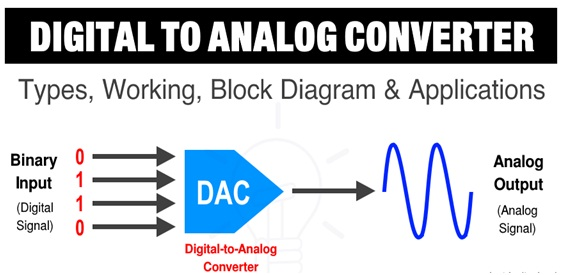
\includegraphics[width=1\textwidth]{Fig 21.jpg}
\caption{Digital to Analog Converter}
\end{figure}
In order to understand the data that we process in a digital domain, we need to convert it into analog domain. An example of that would be the process of audio and video editing. We capture the data using our digital camera and microphone to convert the analog data into digital. We process it using our computers to edit it according to over needs. In order to view our edited work, we use DACs to convert it back into the analog domain to view and listen it through our screen and speakers.
\newpage
\part{Number Systems}
A number is a mathematical value used for counting and measuring objects, and for performing arithmetic calculations. Numbers have various categories like natural numbers, whole numbers, rational and irrational numbers, and so on. Similarly, there are various types of number systems that have different properties, like the binary number system, the octal number system, the decimal number system, and the hexadecimal number system.\\
What are Number Systems?\par
A number system is a system representing numbers. It is also called the system of numeration and it defines a set of values to represent a quantity. These numbers are used as digits and the most common ones are 0 and 1 that are used to represent binary numbers. Digits from 0 to 9 are used to represent other types of number systems.
\section{Definition}
A number system is defined as the representation of numbers by using digits or other symbols in a consistent manner. The value of any digit in a number can be determined by a digit, its position in the number, and the base of the number system. The numbers are represented in a unique manner and allow us to operate arithmetic operations like addition, subtraction, and division.
\section{Types of Number Systems}
There are different types of number systems in which the four main types are:
\begin{itemize}
    \item Binary number system (Base - 2)
\item Octal number system (Base - 8)
\item Decimal number system (Base - 10)
\item Hexadecimal number system (Base - 16)
\end{itemize}
We will study each of these systems one by one, detail.
\begin{figure}[H]
\centering 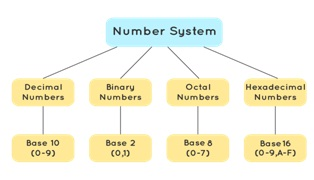
\includegraphics[scale=1]{Fig 22.jpg}
\caption{Types of Number Systems}
\end{figure}
\subsection{Binary}
The binary number system uses only two digits: 0 and 1. The numbers in this system have a base of 2. Digits 0 and 1 are called bits and 8 bits together make a byte. The data in computers is stored in terms of bits and bytes. The binary number system does not deal with other numbers such as 2,3,4,5 and so on. For example: 100012, 1111012, 10101012 are some examples of numbers in the binary number system.\par
The 0s and 1s in binary represent OFF or ON, respectively. In a transistor, a "0" represents no flow of electricity, and "1" represents electricity being allowed to flow. In this way, numbers are represented physically inside the computing device, permitting calculations.\par
A bit (short for binary digit) is the smallest unit of data on a computer; each bit has a single value of either 1 or 0. Executable (ready-to-run) programs are often identified as binary files.
\subsection{Octal}
Octal Number System is a type of number system that has a base of eight and uses digits from 0 to 7. A number system is a system of naming, representing, or expressing numbers in different types of forms. The basic ways of representing numbers are done in four ways i.e. Octal Number System, Binary Number System, Decimal Number System, and Hexadecimal Number System.\par
The octal number system uses eight digits: 0,1,2,3,4,5,6 and 7 with the base of 8. The advantage of this system is that it has lesser digits when compared to several other systems; hence, there would be fewer computational errors. Digits like 8 and 9 are not included in the octal number system. Just as the binary, the octal number system is used in minicomputers but with digits from 0 to 7. For example: 358, 238, 1418 are some examples of numbers in the octal number system.
\subsection{Decimal}
Decimal number system is a base 10 number system having 10 digits from 0 to 9. This means that any numerical quantity can be represented using these 10 digits. Decimal number system is also a positional value system. This means that the value of digits will depend on its position.\\
How to Read Decimal Numbers?\par
In single digits from 0 to 9 the numbers are read as it is. But in the case of two digits, the right digit says what it means, but the left digit means ten times what it says. That is in number 24, 4 is 4, 2 is 20. Altogether forms 24.\par
If we take a three digit number, rightmost digit means what it says; the middle one is ten times the digit, leftmost digit 100 times the digit. Simply if we take number 546, it means (5 x 100) + (4 x 10) + 8 = 54810 \\
(5 x 102) + (4 x 101) + 8 = 54810
\subsection{Hexa-decimal}
Why is it called hexadecimal?\par
The hexadecimal numeral system, often shortened to "hex", is a numeral system made up of 16 symbols (base 16)\par
Hexadecimal is the name of the numbering system that is base 16. This system, therefore, has numerals 0, 1, 2, 3, 4, 5, 6, 7, 8, 9, 10, 11, 12, 13, 14, and 15. That means that two-digit decimal numbers 10, 11, 12, 13, 14, and 15 must be represented by a single numeral to exist in this numbering system.
\newpage
\part{Command List}
The command line is a text interface for your computer. It’s a program that takes in commands, which it passes on to the computer’s operating system to run.\par
From the command line, you can navigate through files and folders on your computer, just as you would with Windows Explorer on Windows or Finder on Mac OS. The difference is that the command line is fully text-based.
\section{Run Commands}
\begin{enumerate}
    \item msconfig 	-	 System Settings.
\item msinfo32 	-	 System Information.
\item resmon 	-	 Resource Monitor.
\item main.cpl 	-	 Mouse Settings.
\item mstsc 	-	 Remote Desktop Service.
\item cmd 	-	 The Command Prompt.
\item explorer 	-	 Windows Explorer.
\item taskmgr 	-	 Task Manager.
\item shutdown 	-	 Windows Shutdown.
\item chkdsk 	-	 Check Disk Utility.
\item cleanmgr 	-	 Clean Disk Manager.
\item dxdiag 	-	 DirectX Options.
\item powershell 	-	 Windows PowerShell Console.
\item winver 	-	 Windows Version.
\item control folders 	-	 Folder Options.
\item diskmgmt.msc 	-	 Disk Manager.
\item eventvwr.msc 	-	 Event Viewer.
\item gpedit.msc 	-	 Local Group Policy Editor.
\item regedit 	-	 Registry Editor.
\item sysdm.cpl 	-	 System Properties.
\item powercfg.cpl 	-	 Power Options.
\item magnify 	-	 Magnifier.
\item charmap 	-	 Windows Character Table.
\item ncpa.cpl 	-	 Network Connections.
\item mrt 	-	 Malware Removal Tool.
\item devmgmt.msc 	-	 Device Manager.
\item netplwiz 	-	 User accounts.
\item services.msc 	-	 Services.
\item appwiz.cpl 	-	 Programs and Components.
\item control 	-	 Control Panel.
\item "." 	-	Open the folder of the current user.
\item osk 	-	 On Screen Keyboard
\item snippingtool 	-	 Scissors.
\item mdsched 	-	 Windows memory checker.
\end{enumerate}		
\section{Command Prompt}
\begin{enumerate}
\item ASSOC          	-	Displays or modifies file extension associations.
\item ATTRIB         	-	Displays or changes file attributes.
\item BREAK          	-	Sets or clears extended CTRL+C checking.
\item BCDEDIT        	-	Sets properties in boot database to control boot loading.
\item CACLS          	-	Displays or modifies access control lists (ACLs) of files.
\item CALL           	-	Calls one batch program from another.
\item CD             	-	Displays the name of or changes the current directory.
\item CHCP           	-	Displays or sets the active code page number.
\item CHDIR          	-	Displays the name of or changes the current directory.
\item CHKDSK         	-	Checks a disk and displays a status report.
\item CHKNTFS        	-	Displays or modifies the checking of disk at boot time.
\item CLS            	-	Clears the screen.
\item CMD            	-	Starts a new instance of the Windows command interpreter.
\item COLOR          	-	Sets the default console foreground and background colors.
\item COMP           	-	Compares the contents of two files or sets of files.
\item COMPACT        	-	Displays or alters the compression of files on NTFS partitions.
\item CONVERT        	-	Converts FAT volumes to NTFS.  You cannot convert the current drive.
\item COPY           	-	Copies one or more files to another location.
\item DATE           	-	Displays or sets the date.
\item DEL            	-	Deletes one or more files.
\item DIR            	-	Displays a list of files and subdirectories in a directory.
\item DISKCOMP       	-	Compares the contents of two floppy disks.
\item DISKCOPY       	-	Copies the contents of one floppy disk to another.
\item DISKPART       	-	Displays or configures Disk Partition properties.
\item DOSKEY         	-	Edits command lines, recalls Windows commands, and creates macros.
\item DRIVERQUERY    	-	Displays current device driver status and properties.
\item ECHO           	-	Displays messages, or turns command echoing on or off.
\item ENDLOCAL       	-	Ends localization of environment changes in a batch file.
\item ERASE          	-	Deletes one or more files.
\item EXIT           	-	Quits the CMD.EXE program (command interpreter).
\item FC             	-	Compares two files or sets of files, and displays the differences between them.
\item FIND           	-	Searches for a text string in a file or files.
\item FINDSTR        	-	Searches for strings in files.
\item FOR            	-	Runs a specified command for each file in a set of files.
\item FORMAT         	-	Formats a disk for use with Windows.
\item FSUTIL         	-	Displays or configures the file system properties.
\item FTYPE          	-	Displays or modifies file types used in file extension associations.
\item GOTO           	-	Directs the Windows command interpreter to a labeled line in a batch program.
\item GPRESULT       	-	Displays Group Policy information for machine or user.
\item GRAFTABL       	-	Enables Windows to display an extended character set in graphics mode.
\item HELP           	-	Provides Help information for Windows commands.
\item ICACLS         	-	Display, modify, backup, or restore ACLs for files and directories.
\item IF             	-	Performs conditional processing in batch programs.
LABEL          	-	Creates, changes, or deletes the volume label of a disk.
\item MD             	-	Creates a directory.
\item MKDIR          	-	Creates a directory.
\item MKLINK         	-	Creates Symbolic Links and Hard Links
\item MODE           	-	Configures a system device.
\item MORE           	-	Displays output one screen at a time.
\item MOVE           	-	Moves one or more files from one directory to another directory.
\item OPENFILES      	-	Displays files opened by remote users for a file share.
\item PATH           	-	Displays or sets a search path for executable files.
\item PAUSE          	-	Suspends processing of a batch file and displays a message.
\item POPD           	-	Restores the previous value of the current directory saved by PUSHD.
\item PRINT          	-	Prints a text file.
\item PROMPT         	-	Changes the Windows command prompt.
\item PUSHD          	-	Saves the current directory then changes it.
\item RD             	-	Removes a directory.
\item RECOVER        	-	Recovers readable information from a bad or defective disk.
\item REM            	-	Records comments (remarks) in batch files or CONFIG.SYS.
\item REN            	-	Renames a file or files.
\item RENAME         	-	Renames a file or files.
\item REPLACE        	-	Replaces files.
\item RMDIR          	-	Removes a directory.
\item ROBOCOPY       	-	Advanced utility to copy files and directory trees
\item SET            	-	Displays, sets, or removes Windows environment variables.
\item SETLOCAL       	-	Begins localization of environment changes in a batch file.
\item SC             	-	Displays or configures services (background processes).
\item SCHTASKS       	-	Schedules commands and programs to run on a computer.
\item SHIFT          	-	Shifts the position of replaceable parameters in batch files.
\item SHUTDOWN       	-	Allows proper local or remote shutdown of machine.
\item SORT           	-	Sorts input.
\item START          	-	Starts a separate window to run a specified program or command.
\item SUBST          	-	Associates a path with a drive letter.
\item SYSTEMINFO     	-	Displays machine specific properties and configuration.
\item TASKLIST       	-	Displays all currently running tasks including services.
\item TASKKILL       	-	Kill or stop a running process or application.
\item TIME           	-	Displays or sets the system time.
\item TITLE          	-	Sets the window title for a CMD.EXE session.
\item TREE           	-	Graphically displays the directory structure of a drive or path.
\item TYPE           	-	Displays the contents of a text file.
\item VER            	-	Displays the Windows version.
\item VERIFY         	-	Tells Windows whether to verify that your files are written correctly to a disk.
\item VOL            	-	Displays a disk volume label and serial number.
\item XCOPY          	-	Copies files and directory trees.
\item WMIC           	-	Displays WMI information inside interactive command shell.
\end{enumerate}		
\section{MS-DOS}
Change the Default Drive\par
To change the default drive, simply type the letter of your choice. The new default will be listed in subsequent DOS prompts.\\
Example:
\begin{itemize}
    \item C\verb=>= A: [enter] - Changes the default drive from C to A.
\item A\verb=>= C: [enter] - Changes the default drive from A to C.
\end{itemize}
The [enter] means that you must press the Enter Key before the format command will execute. [Enter] is required after any DOS command, it is assumed in all commands found below.
CHDIR (CD) Change Directory Command\par
Once you have located the directory you want, you may move from directory to directory using the CD command (change directory)\\
Example:
\begin{itemize}
    \item C\verb=>= cd furniture - Moves you to the directory called 'FURNITURE'
\item C\verb=>= cd \verb=\furniture=\verb=\chairs= - Moves you to the directory called 'CHAIRS' under the directory called 'FURNITURE'.
\item C\verb=>= cd .. - Moves you up one level in the path.
\item C\verb=>= cd \verb=\= - Takes you back to the root directory (c: in this case).
COPY Command
\end{itemize}
The COPY command can be used either to copy files from disk to disk or to create a second copy of a file on a single disk. (There are many more uses of the COPY command, but only the basic operation is discussed here.)\\
Example:
\begin{itemize}
    \item C\verb=>= copy c:kermit.exe a: - Copies the file 'KERMIT.EXE' from the C drive to the A drive and gives it the same name.
\item C\verb=>= copy a:brazil1.dat b:\verb=\=south\verb=\=brazil2.dat - Creates a copy of 'BRAZIL1.DAT' from drive A on drive B, putting it in the 'SOUTH' subdirectory and renaming it 'BRAZIL2.DAT'.
\end{itemize}
The key to use this command correctly is to remember that the first file specified after the COPY command is the source file, the second is the target:ehp1 file. The source is the file to be copied. The target will be the location and name of the new file. If the file name and extension are omitted after the target's drive specification, the new file will have exactly the same name as the source file.\\
Example:
\begin{itemize}
    \item C\verb=>= copy a:myfile.txt b:
\item C\verb=>= copy c:command.com b:com.com
\item C\verb=>= copy b:golly.gee a:whao.boy
\item C\verb=>= copy command.* a:
\item C\verb=>= copy a:mymap.dwg c:\verb=\=maps
\end{itemize}
Note: it is always good practice to us the complete file specifications for both source and target files, Be very sure of yourself before you accept defaults or employ wild-card characters. Otherwise you may end up with some interesting results. Incomplete or incorrect source names may result in errors, such as the command: copy edlin a: myomy.bat. Try it and see what happens.\\
DIR (Directory) Command\par
The DIRECTORY command lists the names and sizes of all files located on a particular disk.
Example:
\begin{itemize}
    \item C\verb=>= dir a: - Shows directory of drive A
\item C\verb=>= dir b: - Shows directory of drive B
\item C\verb=>= dir \verb=\=agis - Shows files in a subdirectory on drive C (default)
\item C\verb=>= dir - Shows directory of drive C
\item C\verb=>= dir /w - Shows directory in wide format, as opposed to a vertical listing.
\end{itemize}
All the files are listed at the screen; you can stop the display by typing CTRL-BREAK. If you ask for a directory on the A or B drives, be sure there is a diskette in the drive and that the diskette has been formatted. If the drive is empty, or if the diskette is unformatted, the DOS will respond with an error message.\\
DIR Options\par
Two little characters, '*' and '?', will make your life with computers much easier. Their use is illustrated below.
Example:
\begin{itemize}
    \item C\verb=>= dir a:*.ex - Lists all files on the A drive with an extension of 'EXE'.
\item C\verb=>= dir b:kermit.* - Lists all files on the B drive with a filename of 'KERMIT'.
\end{itemize}
The asterisk is a wild-card character which allows the user to enter only a limited part of a file specification to find a file. It is useful when you wish to locate a group of files with the same filename or the same extension. On other occasions you may have forgotten part of a file specification. You can use '*' in place of the parts of the specification you have forgotten. Similarly, '?' permits wild-card searches keyed to single characters.\\
Example:
\begin{itemize}
    \item C\verb=>= dir a:labe?.com - Lists all five-letter files with the first four letters 'LABE' and an extension of 'COM'.
\item C\verb=>= dir b:format.c?? - Lists all files with a filename of 'FORMAT' and an extension beginning with 'C'.
\end{itemize}
Wild-card characters can be used in combination.
Example:
\begin{itemize}
    \item C\verb=>= dir a:labe?.* - Lists all five-letter files with the first four letters 'LABE' and any extension.
\item C\verb=>= dir c:*.ex? - Lists all files with an extension beginning with 'EX'.
\end{itemize}	
Experiment with '*' and '?' to improve your ability to find files quickly. These wild-card characters can also be used with several other DOS commands.\\
ERASE Command\par
The ERASE command deletes specified files.\\
Example:
\begin{itemize}
    \item C\verb=>= erase a:myfile.txt - Erases the file MYFILE.TXT from the diskette in the A drive. If no drive specification is entered, the system looks to delete the specified file form drive C (in this case).
\end{itemize}	
File-Naming Conventions\par
Careful file naming can save time. Always choose names which provide a clue to the file's contents. If you are working with a series of related files, use a number somewhere in the name to indicate which version you have created. This applies only to the filename parameter; most of the file extension parameters you will be using are predetermined (or reserved by DOS for certain types of file).\\
Example:
\begin{itemize}
    \item WORLD.DAT - An ATLAS*GRAPHICS file containing data for a world map. The DAT extension is required by ATLAS*GRAPHICS.
\item BRAZIL.BNB - A boundary files of Brazil in binary form.
\item BRIT1.DAT
\item BRIT2.DAT
\item BRIT3.DAT - Three versions of a data file for a map of Britain.
\end{itemize}
FORMAT Command\par
You must format new disks before using them on the IBM computers. The format command checks a diskette for flaws and creates a directory where all the names of the diskette's files will be stored.\\
Example:
\begin{itemize}
    \item C\verb=>= format a: - Formats the diskettes in the A drive.
\item C\verb=>= format b: 
\end{itemize}
MKDIR (MD) Make Directory Command\par
This command creates a new directory.\\
Example:
\begin{itemize}
    \item C\verb=>= mkdir mine - Creates a directory called 'MINE'
\end{itemize}
Rebooting the computer (Ctrl-Alt-Del)\par
In some cases, when all attempts to recover from a barrage of error messages fails, as a last resort you can reboot the computer. To do this, you press, all at once, the control, alternate and delete.\\
RENAME (REN) Command\par
The RENAME command permits users to change the name of a file without making a copy of it.\\
Example:
\begin{itemize}
    \item C\verb=>= ren a:goofy.txt pluto.txt - Changes the name of ‘GOOFY.TXT’ on the A drives to 'PLUTO.TXT'.
\end{itemize}
This command is very simple to use, just remember two points:
\begin{enumerate}
    \item The file name and extension must be complete for the source file and no drive specification is given for the target.
    \item Renaming can only occur on a single disk drive (otherwise COPY must be used).
\end{enumerate}
RMDIR (RD) Remove Directory Command\par
This command removes a directory. It is only possible to execute this command if the directory you wish to remove is empty.\\
Example:
\begin{itemize}
    \item C\verb=>= rd mine - Removes directory called 'MINE'.
\end{itemize}
Stop Execution (Ctrl-Break)\\
If you wish to stop the computer in the midst of executing the current command, you may use the key sequence Ctrl-Break. Ctrl-Break does not always work with non-DOS commands. Some software packages block its action in certain situations, but it is worth trying before you re-boot.
\newpage
\part{Microsoft Office}
Microsoft Office is a set of computer applications mainly used for business or office purposes. First introduced in 1990, Office software is made by the Microsoft Corporation. MS Office helps simplify basic office tasks and improve work productivity.\par
Microsoft Office is a suite of applications designed to help with productivity and completing common tasks on a computer. You can create and edit documents containing text and images, work with data in spreadsheets and databases, and create presentations and posters.\par
Microsoft Word is used for writing books, letters, resumes, applications, or any other documentation work. Microsoft Excel is used for calculations, data analyses  data consolidation. Microsoft Powerpoint is used to present the data summary in the form of slides. This Microsoft Office course is a complete guide to all three above-mentioned MS office products. In this course of Microsoft office, you will be able to learn the all above-mentioned uses of Microsoft Word, Microsoft PowerPoint and Microsoft Excel.\par
This Microsoft office course is All in one complete MS office training from beginner to expert level. Microsoft office is the need of everyone so If you are working in any field like engineering, auditing, data analyzing, data entry, or if you are a student, teacher, or researcher or are working in the field where any of these three products of Microsoft Office are used you can choose this course to gain the skill as per your requirement.
\section{MS Office}
\begin{itemize}
    \item Microsoft Word
\item Microsoft Excel
\item Microsoft PowerPoint
\end{itemize}
\subsection{Microsoft Word}
\begin{figure}[H]
\centering 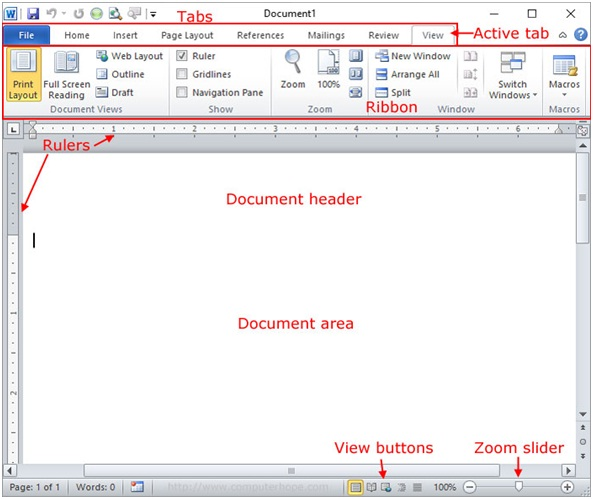
\includegraphics[width=0.5\textwidth]{Fig 23.jpg}
\caption{MS Word Window}
\end{figure}
Microsoft Word allows you to create professional-quality documents, reports, letters, and résumés. Unlike a plain text, editor, Microsoft Word has features including spell check, grammar check, text and font formatting.\\
Microsoft Word is a computer application program written by Microsoft. It is mainly used to design text for presentation.\\
Our MS Word tutorial includes all topics of MS Word such as save the document, correct error, word count, font size, font style, apply a style, customize a style, page size, page margin, insert header and footer and more.
\begin{itemize}
    \item To create business documents having various graphics including pictures, charts, and diagrams.
\item To store and reuse readymade content and formatted elements such as cover pages and sidebars.
\item To create letters and letterheads for personal and business purpose.
\item To design different documents such as resumes or invitation cards etc.
\item To create a range of correspondence from a simple office memo to legal copies and reference documents.
\end{itemize}
Getting Familiar with Microsoft Word\\
Microsoft Word is a word processing software package. You can use it to type letters, reports, and other documents. This lesson introduces you to the Word window. You use the Word window to interact with Microsoft Word.
\begin{itemize}
    \item The Microsoft Word Title Bar
\item The Microsoft Word Menu Bar
\item Microsoft Word Toolbars
\item The Ruler
\item Document View 
\item Text Area 
\item Exiting Microsoft Word 
\end{itemize}
What does the Microsoft Word editor look like? \\
The right figure gives an overview of a Microsoft Word 2010 document.	\\
Working with the Word environment\\
All recent versions of Word include the Ribbon and the Quick Access Toolbar, where you'll find commands to perform common tasks in Word, as well as backstage view.\\
The Ribbon
\begin{figure}[H]
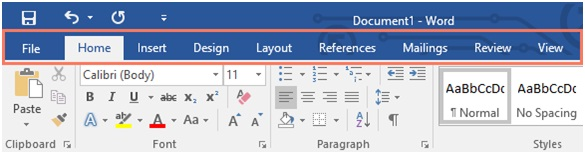
\includegraphics[width=1\textwidth]{Fig 24.jpg}
\caption{Ribbons in MS Word}
\end{figure}
Word uses a tabbed Ribbon system instead of traditional menus. The Ribbon contains multiple tabs, which you can find near the top of the Word window.
\begin{figure}[H]
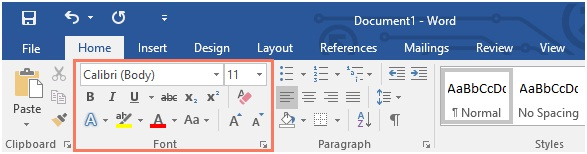
\includegraphics[width=1\textwidth]{Fig 25.jpg}
\caption{Font Group in MS Word}
\end{figure}
Each tab contains several groups of related commands. For example, the Font group on the Home tab contains commands for formatting text in your document.\par
Some groups also have a small arrow in the bottom-right corner that you can click for even more options.
\begin{figure}[H]
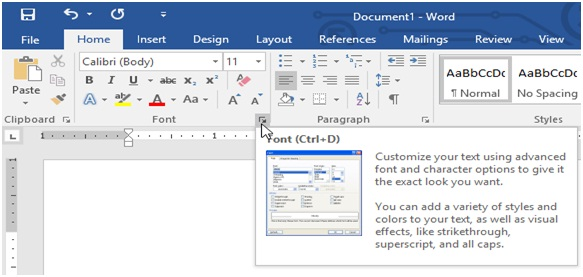
\includegraphics[width=1\textwidth]{Fig 26.jpg}
\caption{Expanded Font Settings}
\end{figure} 

MS Word shortcut keys
\begin{itemize}
\item Ctrl + A -- Select all contents of the page.
\item Ctrl + B -- Bold highlighted selection.
\item Ctrl + C -- Copy selected text.
\item Ctrl + X -- Cut selected text.
\item Ctrl + N -- Open new/blank document.
\item Ctrl + O -- Open options.
\item Ctrl + P -- Open the print window.
\item Ctrl + F -- Open find box.
\item Ctrl + I -- Italicize highlighted selection.
\item Ctrl + K -- Insert link.
\item Ctrl + U -- Underline highlighted selection.
\item Ctrl + V -- Paste.
\item Ctrl + Y -- Redo the last action performed.
\item Ctrl + Z -- Undo last action.
\end{itemize}
	
\subsection{MS Excel}    
\begin{figure}[H]
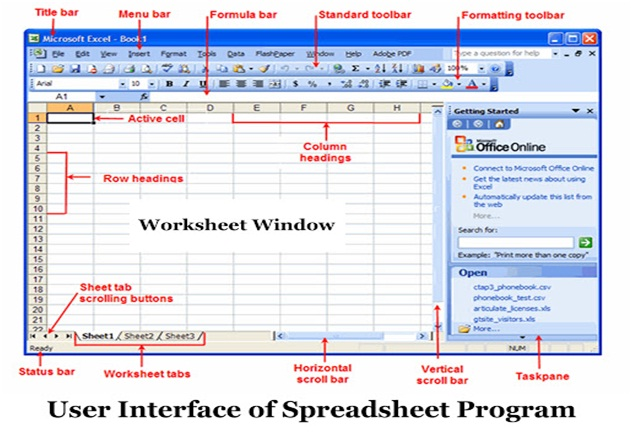
\includegraphics[width=1\textwidth]{Fig 27.jpg}
\caption{MS Excel Window}
\end{figure}
Excel is an incredibly powerful tool for getting meaning out of vast amounts of data. But it also works really well for simple calculations and tracking almost any kind of information. The key for unlocking all that potential is the grid of cells. Cells can contain numbers, text, or formulas. You put data in your cells and group them in rows and columns. That allows you to add up your data, sort and filter it, put it in tables, and build great-looking charts. Let’s go through the basic steps to get you started.\par
Microsoft Excel is program for data analysis and documentation. It is a spreadsheet program, which contains a number of columns and rows, where each intersection of a column and a row is a “cell.” Each cell contains one point of data or one piece of information. By organizing the information in this way, you can make information easier to find, and automatically draw information from changing data.\\
EXCEL FEATURES\par
There are a number of features that are available in Excel to make your task easier. Some of the main features are: AutoFormat\par
Lets you to choose many preset table formatting options. \\
AutoSum \par
Helps you to add the contents of a cluster of adjacent cells. 
List AutoFill
Automatically extends cell formatting when a new item is added to the end of a list.
Home
Comprises options like font size, font styles, font colour, background colour, alignment, formatting options and styles, insertion and deletion of cells and editing options
Insert
Comprises options like table format and style, inserting images and figures, adding graphs, charts and sparklines, header and footer option, equation and symbols
Page Layout
Themes, orientation and page setup options are available under the page layout option
Formulas
Since tables with a large amount of data can be created in MS excel, under this feature, you can add formulas to your table and get quicker solutions.
Data
Adding external data (from the web), filtering options and data tools are available under this category
Review
Proofreading can be done for an excel sheet (like spell check) in the review category and a reader can add comments in this part 
View
Different views in which we want the spreadsheet to be displayed can be edited here. Options to zoom in and out and pane arrangement are available under this category
MS excel Formula
SUM
As the name suggests, gives the total of the selected range of cell values. It performs the mathematical operation which is addition. Here’s an example of it below:
\begin{figure}[H]
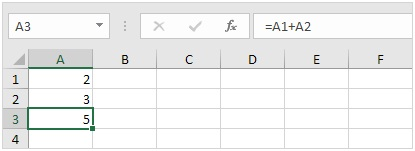
\includegraphics[width=1\textwidth]{Fig 28.jpg}
\caption{Sum function shown in Formula Bar of MS Excel}
\end{figure}
AVERAGE
This function focuses on calculating the average of the selected range of cell values. As seen from the below example, to find the avg of the total sales, you have to simply type in “AVERAGE(C2, C3, C4)”.
\begin{figure}[H]
\centering 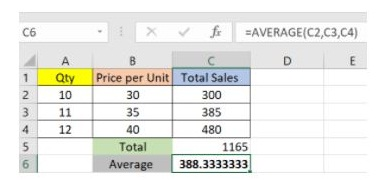
\includegraphics[scale=1.2]{Fig 29.jpg}
\caption{Calculation of Average in MS Excel}
\end{figure}
\subsection{MS PowerPoint}
PowerPoint is a presentation program developed by Microsoft that creates a slide show of important information, charts, and images for a presentation. It is most often used for business and school presentations.\par
It is widely used, and considered the "standard" for presentation software. If you create a PowerPoint presentation, it's more likely it will be easier for others to open and view.\par
It includes many optional presentation features, including slide transitions, animations, layouts, templates, and more.\par
It offers the option to export its slides to alternative file formats, including GIF and JPG images, MPEG-4 video, PDF, RTF (rich text format), WMV (Windows Media Video), and PowerPoint XML.\par
PowerPoint (PPT) is a powerful, easy-to-use presentation graphics software program that allows you to create professional-looking electronic slide shows. 
\begin{figure}[H]
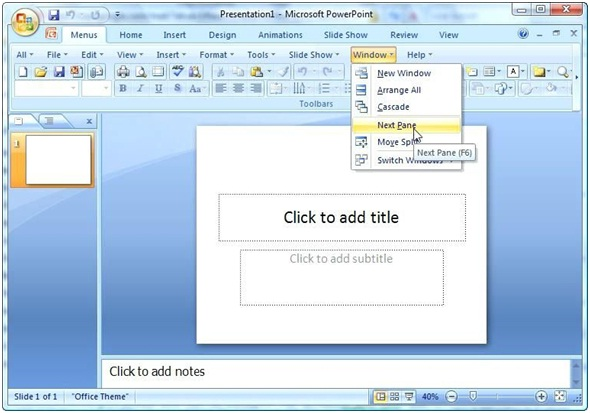
\includegraphics[width=1\textwidth]{Fig 30.jpg}
\caption{MS Powerpoint Window}
\end{figure}
PowerPoint template\par
The most important part of a PowerPoint template is the Master slide. The Master slide is the top slide you see when you open the presentation’s Slide Master View. This is where you would add a logo or any graphics you want repeated on all slides, set the background for all the individual slide layouts, decide if your headlines should be all capitalized, what your bullets should look like, the spacing of text, where your footers and slide numbers should be placed etc\\
Defined Theme Font\par
PowerPoint comes with the capability to define theme fonts – a font for headings and a font for the body text. The theme fonts automatically define the text in any placeholder, graph, text box, SmartArt etc in a presentation. The theme fonts that have been defined for a presentation can be seen at the top of the font menu on the Home tab.\\
Theme Effects\par
PowerPoint comes with a set of theme effects that can be applied to a file or a template. The theme effects influences fills, lines, shadows, bevels and special effects of graphic objects created in PowerPoint each with a different set of effects. Once applied, the variants of that effect theme is available to the users when they are creating shapes, tables, SmartArt and charts so make sure you have applied an effect theme where all variants in the effect theme fit your brand.\\
Insert a picture from your computer on your slide
\begin{wrapfigure}{r}{5cm}
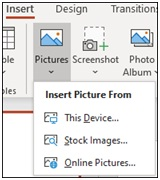
\includegraphics[width=5cm,height=3cm]{Fig 31.jpg}
\caption{Inserting Pictures}
\end{wrapfigure}
Click where you want to insert the picture on the slide.
On the Insert tab, in the Images group, click Pictures and then click This Device.
\begin{itemize}
\item In the dialog box that opens, browse to the picture that you want to insert, click that picture, and then click Insert.
\item Insert and play a video file from your compute
\item Embed a video stored on your PC
\item In Normal view, click the slide that you want the video to be in.
\item On the Insert tab, click the arrow under Video, and then click Video on My PC.
\item In the Insert Video box, click the video that you want, and then click Insert.
\end{itemize}
Link to a video stored on your PC\par
To help prevent broken links, we recommend copying the video into the same folder as your presentation, and then linking to it there.\\
\begin{figure}[H]
\centering 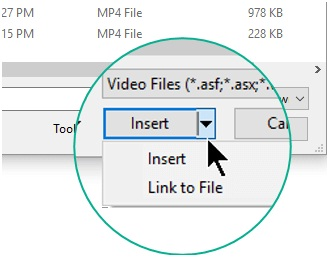
\includegraphics[scale=1]{Fig 32.jpg}
\caption{Inserting a Video file}
\end{figure}
In Normal view, click the slide where you want the link to the video to be in.\\
On the Insert tab, click the arrow under Video, and then click Video on my PC.\\
In the Insert Video box, click the file that you want to link to, click the down arrow next to the Insert button, and then click Link to File.
\newpage
\part{Basics of Internet}
The Internet is a worldwide telecommunications system that provides connectivity for millions of other, smaller networks; therefore, the Internet is often referred to as a network of networks. It allows computer users to communicate with each other across distance and computer platforms.\par
The Internet is the collection of the many different systems and protocols.\par
The Internet is a global collection of computer networks that are linked together by devices called routers and use a common set of protocols for data transmission known as TCP/IP (transmission control protocol / Internet protocol). The primary purpose of the Internet is to facilitate the sharing of information. There are many different tools used on the Internet to make this possible. Some of the more common tools include email, list servers, newsgroups, FTP, and the World Wide Web. Probably the most popular of all Internet tools is the World Wide Web we are going to explore the fascinating and ever-changing world of the Internet. The Internet is the largest computer network in the world, connecting more than a billion computer users. The Internet is most often used for three main purposes:
\begin{enumerate}
\item Communication
\item Buying and selling (e-commerce)
\item Searching for information
\end{enumerate}
One of the most important things you need to know about the Internet is that it is a self-publishing medium, which means that no one is in charge of the content found on it. Anyone can publish anything on the Internet, whether the information is true or not. Later in this Learning Unit, you will learn some tips for evaluating the information you find on websites.
Ways to Connect To Internet\\
The different ways in which one can connect to the Internet are discussed below in brief:
\begin{itemize}
\item Dial-Up – In such connections, users are required to link their phone line to a computer to access the Internet. Under this connection, the user cannot make or receive phone calls through tier home phone service
\item Broadband – Provided either through cable or phone companies, Broadband is a high-speed internet connection which is widely used today
\item Wireless Connection – Wi-fi and Mobile service providers fall under this category. Internet connectivity is made via radio waves and the Internet can be connected anywhere, irrespective of the location. Given below are a few examples of wireless connection:
\item Wi-fi – Wireless Fidelity or wi-fi allows high-speed internet connectivity without the use of wires
\item Mobile Phones – All smartphones are now equipped with an option for Internet connectivity which can be availed using Internet vouchers and packs. No external connection or wire is required for these
\item Satellite – Where broadband connections are unavailable, satellites are used for wireless Internet connectivity
\item Integrated Services Digital Network – ISDN allows users to sent audio or video data using telephone lines
\end{itemize}
Intentionally or unintentionally, Internet usage is a part in the day to day lives of every individual. The Internet has made lives easy and comfortable, but at the same time made human being dependable for the smallest or biggest of information. Discussed below are the uses of the internet, along with a few cons that it brings along.
\begin{figure}[H]
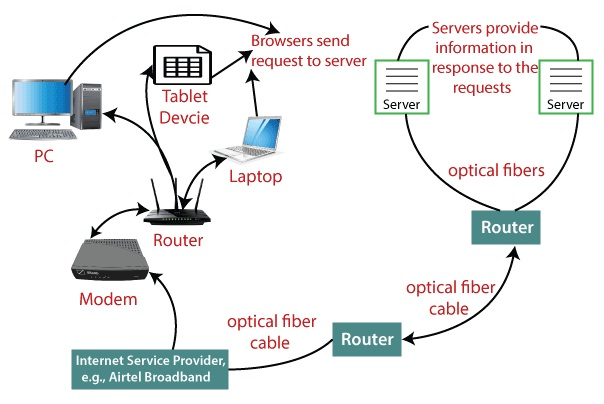
\includegraphics[width=1\textwidth]{Fig 33.jpg}
\caption{Working of the Internet}
\end{figure}
Pros of Internet
\begin{itemize}
    \item Easy Access to Information – Information on anything and everything are available online. The Internet makes it convenient to learn about new things at any point in time and get details on various subjects, irrespective of time and place.
\item Platform for Online Education – With the advanced technology, even students and adults wish to learn new things and gaining knowledge at various online portals has become more accessible
\item Job Hunting – Employers can look for employees on the internet and the job seekers can apply online for jobs using the Internet
\item Platform to become an Entrepreneur – Today, thousands of people have started their own websites and getting good business and users/customers by making their own websites and selling products or services. This has become accessible due to Internet connectivity
\item Visual and Graphical Representation of Things – Various researches have shown that a person tends to get more engaged with a graphical representation of things. Internet has made this facility also convenient for both user and creator 
\item Reduced the parameter of Distance – Social media has reduced the distance between people as communication has become much easier because of Internet connection.
\end{itemize}
With the Internet being an extremely essential part of daily life, it is important that a person is well aware of the disadvantages of the Internet and its excess usage.\\
Cons of Internet
\begin{itemize}
    \item Dependency – The dependency of people for looking things and information online has increased massively since the introduction of Internet and its easy access
\item Cyber Crime – People do not just use internet for learning purposes, cybercrime has also been at a distinctive high because of effortless availability of resources
\item Distraction – People can easily find online games, interesting information, etc. online which may be a cause of distraction for may
\item Bullying and Trolls – Online platforms are being used for unethical practices like bullying people and trolling them
\end{itemize}
Modem-ISP\\
Modem\\
A modem or broadband modem is a hardware device that connects a computer or router to a broadband network. For example, a cable modem and DSL modem are two examples of these types of Modems.\par
Short for modulator/demodulator, a modem is a hardware device that allows a computer to send and receive information over telephone lines. When sending a signal, the device converts ("modulates") digital data to an analog audio signal, and transmits it over a telephone line. Similarly, when an analog signal is received, the modem converts it back ("demodulates" it) to a digital signal.
 \begin{figure}[H]
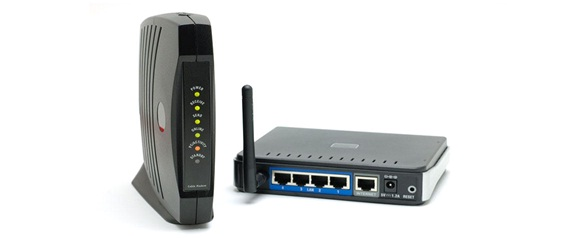
\includegraphics[width=1\textwidth]{Fig 34.jpg}
\caption{Modem(Modulator/Demodulator)}
\end{figure}
ISP\\
Internet service provider (ISP), company that provides Internet connections and services to individuals and organizations. In addition to providing access to the Internet, ISPs may also provide software packages (such as browsers), e-mail accounts, and a personal Web site or home page. ISPs can host Web sites for businesses and can also build the Web sites themselves. ISPs are all connected to each other through network access points, public network facilities on the Internet backbone.\\
Internet Service Provider (ISP):\\
Internet Service Providers are companies that connect you to the Internet – for a fee, of course. ISPs are available on a local, state, and national level. Large communication companies control access to the main lines of the Internet structure. They, in turn, supply Internet access to the smaller ISPs, who pass this along to the consumer. Not all ISPs offer all methods of connection to the Internet. Make sure the ISP you select offers service that corresponds to your connection method and hardware.\\
E-Mail\\
E-mail, in full electronic mail, messages transmitted and received by digital computers through a network. An e-mail system allows computer users on a network to send text, graphics, sounds, and animated images to other users.\par
On most networks, data can be simultaneously sent to a universe of users or to a select group or individual. Network users typically have an electronic mailbox that receives, stores, and manages their correspondence. Recipients can elect to view, print, save, edit, answer, forward, or otherwise react to communications. Many e-mail systems have advanced features that alert users to incoming messages or permit them to employ special privacy features. Large corporations and institutions use e-mail systems as an important communication link between employees and other people allowed on their networks. E-mail is also available on major public online and bulletin board systems, many of which maintain free or low-cost global communication networks.
\section{Working of E-mail}
\begin{figure}[H]
\centering 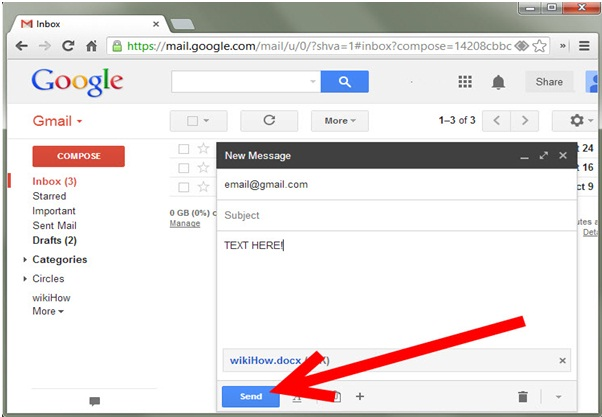
\includegraphics[scale=1]{Fig 35.jpg}
\caption{Sending an E-Mail}
\end{figure}
Email working follows the client server approach. In this client is the mailer i.e. the mail application or mail program and server is a device that manages emails.\par
Following example will take you through the basic steps involved in sending and receiving emails and will give you a better understanding of working of email system:
\begin{itemize}
\item Suppose person A wants to send an email message to person B.
\item Person A composes the messages using a mailer program i.e. mail client and then select Send option.
\item The message is routed to Simple Mail Transfer Protocol to person B’s mail server.
\item The mail server stores the email message on disk in an area designated for person B.
The disk space area on mail server is called mail spool.
\item Now, suppose person B is running a POP client and knows how to communicate with B’s mail server.
\item It will periodically poll the POP server to check if any new email has arrived for B.As in this case; person B has sent an email for person B, so email is forwarded over the network to B’s PC. This is message is now stored on person B’s PC.
\end{itemize}
\section{Worldwide web and Search engines}
 World Wide Web (WWW) is made up of a lot of interconnected computers (via phone lines, cables, or satellites). Some of these computers are designed to serve out WebPages. These computers are called web servers, which are usually running 24/7. Other computers, like the one you are using to read this text, are called clients. Client computers make requests to server computers, like asking for a web page and its associated graphics. The server computer responds by feeding (or serving) the web page data back to the client.\par
The Internet is often confused with the World Wide Web. The Internet consists of a wide range of technologies including email, file data transfer, protocols (communications infrastructure) as well as the Web. The World Wide Web is just one component of the Internet.
\subsection{Web Browsers}
Web browsers are computer programs that are installed on client computers to request web page files from server computers. It’s the program you’re using to access this website and read this text. Once a request is made via the browser (by clicking a link or entering a web address in the “address bar”), the web server sever sends the requested data back to the browser. The browser then interprets the data and displays it on the screen.\par
Popular web browsers include Firefox, Chrome, Opera, etc., each of these browsers differs somewhat in terms of features, but their purpose is the same. They’re all meant to request and present web pages to the user.\\
“Mobile browsers” are web browsers designed for use on mobile devices like PDAs and cell phones.
\section{Website}
A website is made up of a collection of files sitting on a web server. These files usually include:
\begin{itemize}
\item Image and/or video files
\item Text files that tell the web browser how to layout the page and what text to include
\item Script files (small programs) that add functionality or effects to the webpage
\end{itemize}
\subsection{Website Hosting}
The files that make up your website have to be put somewhere that people can access. This somewhere is a computer running web server software.  The server takes incoming user requests and returns your website files to their browser. Web hosts are companies that rent space on their servers for you to store your website files on. The web host takes care of the necessary computer hardware, software and connections.
\subsection{Website Address}
Let’s say you have a website, how can people reach it? One answer is, by entering your website address (or “URL” in nerd-speak) into your browser’s address bar. A website has to have a unique address so that it can be found. Just as real world home addresses are unique to avoid confusion, website addresses have to be unique also.\\
How do you get a unique address?\\
By registering a domain name. Examples of domain names are “ibm.com” and “wikipedia.org”. Our domain name is “helpsme.com”. The helpsme.com domain name is mapped to the server that stores the files that makes up this website.
An organization named ICANN coordinates these domain names across the world. This is necessary so that when you type an address into your browser, you reach the website you were looking for.
\subsection{A search engine} 
It is software accessed on the Internet that searches a database of information according to the user's query. The engine provides a list of results that best match what the user is trying to find. Today, there are many different search engines available on the Internet, each with its own abilities and features. The first search engine ever developed is considered Archie, which was used to search for FTP files, and the first text-based search engine is considered Veronica. Currently, the most popular and well-known search engine is Google. Other popular search engines include AOL, Ask.com, and Yahoo.\\
How to access a search engine?\\
For users, a search engine is accessed through a browser on their computer, smartphone, tablet, or another device. Today, most new browsers use an omnibox, which is a text box at the top of the browser. The omnibox allows users to type in a URL or a search query. You can also visit one of the major search engines' home page to perform a search.
\subsection{Upload and download}
While exploring the Internet, you’ve probably encountered the terms downloading and uploading. Downloading means receiving data or a file from the Internet on your computer. Uploading means sending data or a file from your computer to somewhere on the Internet.\\
These terms describe activities you may have already learned how to do. If you've ever opened an example document in one of our tutorials, you've downloaded that file. If you’ve ever shared a photo you took on Facebook or another social media site, you've uploaded that photo.
\begin{figure}[H]
\centering 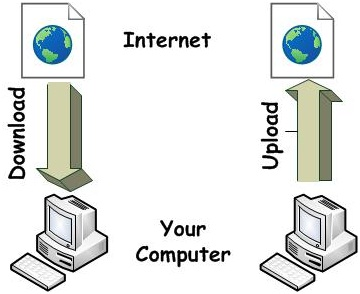
\includegraphics[scale=1]{Fig 36.jpg}
\caption{Download/Upload Representation}
\end{figure}
\noindent Downloading\\
Usually, when you download a file you will start the download by clicking a link to that file. Many of our tutorials contain links to files, like this:\\
If you click the link, your browser should prompt you to select one of two methods for downloading the file.
\begin{itemize}
\item Open with will download the file and load it immediately in the specified program.
\item Save File will download it and save it to your hard drive.
\item Download = save. You're taking data from elsewhere and putting it onto your device, essentially bringing it "down" from the internet.
\item Downloading something from the web means that you're transferring data from the other location to your own device, whether it be your phone, computer, tablet, smartwatch, etc
\end{itemize}
All sorts of information can be downloaded from the web: books, movies, software, etc. For example, you can download movies to your phone to watch while you're on the go, which means that the actual data that makes up the movie is transferred from the site you got it from and saved to your phone, making it locally available.\\
Uploading\\
Upload = send. You can think of it like loading the data "upward" to the cloud/internet.\par
When you upload something to a website, another user's computer, a network location, etc., you're sending data from your device to the other device. Files can be uploaded to a server, such as a website, or directly to another device, like when using a file transfer utility.\par
For example, if you upload an image to Facebook, you're sending the picture from your device to the Facebook website. The file started with you and ended up somewhere else, so it's considered an upload from your perspective.\par
This is true for any transfer like this, no matter the file type or where it's going. You can upload documents to your teacher via email, upload a video to YouTube, upload music to your online music collection, etc.\par
Difference between Downloading and Uploading:\\
Downloading	Uploading\\
It is a procedure of copying files from the web server to the machine.	It is a Procedure for copying data from the device to the web server.\\
Memory is required in the user’s device to downloading anything.	Memory is required in the web server to upload anything.\\
Downloading speed is Comparatively High.	Uploading speed is Comparatively low.\\
Data travels from the Web server to the user’s device.	Data travels from user’s device to the web server.
\newpage
\part{Maintenance and Internet Security}
Run operating system updates at least once a week.
Updates to your system software are released on a regular basis to fix bugs, patch security vulnerabilities and improve system performance. Microsoft, for example, releases new critical updates on the second Tuesday of each month. In addition to fixing problems with the software, some software updates introduce new features to enhance system usability. Installing these updates on a regular basis ensures that your system software is current and running at its optimal level.\\
Allow your system to shutdown completely.\\
Let your computer shutdown completely before cutting its power. Improperly shutting down your computer can potentially corrupt files that it uses in the background to operate. To ensure that these files are closed properly, use Shut Down in the Start menu, or hit Alt-F4 to shut down your PC gracefully. For Mac, select Shut Down from the Apple Menu. On some Macs, you may be prompted to Shut Down by pressing the power button.\\
Run virus and malware scans regularly.\\
Be sure you have an Anti-Virus program installed and keep it updated. Install and regularly run spyware detection software in addition to your Anti-Virus program. Spybot, Ad-Aware, or Windows Security Essentials are some programs that will detect many malicious programs that anti-virus might miss.\\
Keep your computer’s hardware clean.\\
Dust can clog fans and cause a computer to overheat, so it is important keep it clean and free of dust and debris. You can minimize dust accumulation by keeping your computer elevated from the floor, especially away from pets and cigarette smoke.\\
Perform regular backups of personal files.\\
To ensure that you do not lose important data in the case that something does happen to harm your computer, it’s important to perform regular backups of personal files. Save your files to the cloud or copy to external hard disk to prevent data loss.
\section{Security}
\subsection{Virus}
Virus stands for Vital Information Resources under Siege. It refers to the type of malicious software or malware that can cause damage to your data, files, and software through replication.\\
Types of Viruses\\
The main types of computer virus are as follows:
\begin{itemize}
\item Boot Sector Virus
\item Direct Action Virus
\item Multipartite Virus
\item Polymorphic Virus
\item Resident Virus
\item File Infector Virus
\end{itemize}
Examples of Viruses\\
Given below are a few examples of a computer virus:
\begin{itemize}
\item Storm Worm
\item CryptoLocker
\item Slammer
\item Creeper
\item Netsky
\end{itemize}
Here’s a list of the common types of malware and their malicious intent:\\
\begin{enumerate}
\item Trojans - A Trojan (or Trojan horse) disguises itself as legitimate software with the purpose of tricking you into executing malicious software on your computer.
\item Spyware - Spyware invades your computer and attempts to steal your personal information such as credit card or banking information, web browsing data, and passwords to various accounts.
\item Adware - Adware is unwanted software that displays advertisements on your screen. Adware collects personal information from you to serve you with more personalized ads.
\item Rootkits - Rootkits enable unauthorized users to gain access to your computer without being detected.
\item Ransomware - Ransomware is designed to encrypt your files and block access to them until a ransom is paid.
\item Worms - A worm replicates itself by infecting other computers that are on the same network. They’re designed to consume bandwidth and interrupt networks.
\item Keyloggers - Keyloggers keep track of your keystrokes on your keyboard and record them on a log. This information is used to gain unauthorized access to your accounts.
\end{enumerate}
\subsection{Anti-Virus}
An anti-virus is software which comprises programs or set of programs which can detect and remove all the harmful and malicious software from your device. This anti-virus software is designed in a manner that they can search through the files in a computer and determine the files which are heavy or mildly infected by a virus.\\
Given below is a list of few of the major antivirus software which is most commonly used:
\begin{itemize}
\item Norton Antivirus
\item F-Secure Antivirus
\item Kaspersky Antivirus
\item AVAST Antivirus
\item Comodo Antivirus
\item McAfee Antivirus
\end{itemize}
\section{Online safety tips}
\begin{itemize}
\item Be alert - Use common sense and think twice before clicking links, opening attachments or responding to emails. Remember, if something sounds too good to be true, it probably is.
\item Throw it out if in doubt - Be wary of emails that require "immediate action" or ask for personal information. Delete any messages that look suspicious.
\item Protect your passwords - Create different passwords for different sites and use a combination of letters, numbers and symbols to make them hard to guess. And never share your passwords with anyone, including close friends.
\item Keep apps and software up-to-date - Set up automatic updates for your computer and mobile devices and regularly restart them to give them a chance to complete the update process.
\item Limit activities on public Wi-Fi - Never use public Wi-Fi to access or enter sensitive information, such as online banking, and consider using a virtual private network (VPN) to lock down your connection.
\item Avoid over sharing on social media. Sharing too much information, such as indicating when you're on vacation or away from home, can make you an easy target for burglary. Also, adjust privacy settings on your accounts and only friend people you know.
\item Be a savvy online shopper - Always use a secure or private Wi-Fi network to shop online. Look for the lock symbol next to the web address before entering payment information and use a credit card or secure payment site like PayPal—not a debit card—to complete transactions.
\item Use two-factor authentication - If a site or app offers you the ability to set up two-factor authentication when signing in, do it. This extra layer of security will require you to verify your identity twice before you can access sensitive information.
\item Back up files and data on a regular basis 	Set up automatic backups of your device and store the backup to a cloud service or external hard drive.
\item Be a good online citizen 	What you do online has the potential to affect everyone—at home, at school and around the world—so always be courteous and practice good online etiquette.
\end{itemize}
\newpage
\part{DBMS}
\section{History}
The first DBMS was developed in the early 1960s when Charles Bachman created a navigational DBMS known as the Integrated Data Store. Shortly after, IBM developed Information Management System (IMS), a hierarchical DBMS designed for IBM mainframes that's still used by many large organizations today.\par
The next major advancement came in 1971 when the Conference/Committee on Data Systems Languages (CODASYL) standard was delivered. Integrated Database Management System is a commercial implementation of the network model database approach advanced by CODASYL.\par
But the DBMS market changed forever as the relational model for data gained popularity. Introduced by Edgar Codd of IBM in 1970 in his seminal paper "A Relational Model of Data for Large Shared Data Banks," the RDBMS soon became the industry standard. The first RDBMS was Ingres, developed at the University of California, Berkeley by a team led by Michael Stonebraker in the mid-1970s. At about the same time, IBM was working on its System R project to develop an RDBMS.\par
In 1979, the first successful commercial RDBMS, Oracle, was released, followed a few years later by IBM's Db2, Sybase SQL Server and many others.\par
In the 1990s, as object-oriented (OO) programming became popular, several OO database systems came to market, but they never gained significant market share. Later in the 1990s, the term NoSQL was coined. Over the next decade, several types of new non-relational DBMS products, including key-value, graph, document and wide-column store, were grouped into the NoSQL category.\par
Today, the DBMS market is dominated by RDBMS, but NewSQL and NoSQL database systems continue to grow in popularity.
\section{Benefits}
One of the biggest advantages of using a DBMS is that it lets users and application programmers access and use the same data concurrently while managing data integrity. Data is better protected and maintained when it can be shared using a DBMS instead of creating new iterations of the same data stored in new files for every new application. The DBMS provides a central store of data that multiple users can access in a controlled manner.\par
Central storage and management of data within the DBMS provide the following:
\begin{itemize}
\item data abstraction and independence;
\item data security;
\item a locking mechanism for concurrent access;
\item an efficient handler to balance the needs of multiple applications using the same data;
\item the ability to swiftly recover from crashes and errors;
\item strong data integrity capabilities;
\item logging and auditing of activity;
\item simple access using a standard API; and
\item Uniform administration procedures for data.
\end{itemize}
Another advantage of a DBMS is that database administrators (DBAs) can use it to impose a logical, structured organization on the data. A DBMS delivers economy of scale for processing large amounts of data because it's optimized for such operations.
\newpage
\part{Telemedicine}
\section{Introduction}
Telemedicine is a process of sharing health related information for diagnosis from one place to another via phone calls, video calls and emails. The information related to health is exchanged in order to treat patients remotely. One can stay home, call a local doctor to help the diagnosis process explained by specialist doctor from anywhere across the world.\par
Telemedicine has been around for over forty years. It's a booming field. It can be difficult to get an appointment with primary care doctors and specialists. Waiting lists can be long, and even getting a referral doesn't guarantee a quick appointment. Telemedicine can help you get closer to your doctor more effectively.
\section{Types of telemedicine}
\subsection{Store-and-forward}
Store-and-forward telemedicine goes beyond the need for doctors to meet in person with their patients. Instead, patient information such as medical images and biosignals can be sent to specialists on demand as they are obtained from the patient. This practice is common in the medical fields of dermatology, radiology, and pathology. With the right structure and care, storing and transferring telemedicine saves time and allows doctors to serve you better at their services. However, this form of telemedicine relies on medical history reports and documented information or images rather than physical examinations, which can lead to complications such as misdiagnosis.
\subsection{Remote Monitoring}
Remote monitoring is a process of analyzing clinical signs or symptoms and health remotely. On a large scale used in management of chronic diseases such as cardiovascular disease, diabetes mellitus, and asthma. It is cost efficient and patient satisfactory, also frequent monitoring can be done.
\subsection{Real-time interactive services}
Interactive services can provide immediate advice to patients who require medical attention. There are several different mediums utilized for this purpose, including phone, online, and home visits. A medical history and consultation about presenting symptoms can be undertaken, followed by an assessment similar to that which is usually conducted during face-to-face appointments.
\newpage
\part{Hospital Information System}
\section{Definition}
Hospital information allows the collection of all data for the treatment of patients, maintaining their medical records, billing services provided to insurance companies and patients, receiving employees working hours and paying them, ordering and paying for supplies and services, recording and reporting financial data, scheduling appointments, recording documentation of patient treatments and making them available to future providers. They are the basic functions of a hospital information system. The are many nuances to some of these functions.\par
Basically the system tracks all information needed to keep the hospital running. The is a general distinction between the clinical and financial functions. Many hospitals use specialized that perform a subset of these functions with higher functionality than a single system that does it all.

\section{Architecture}
There are many ways that you can practice medical architecture. Participating in a team that designs hospitals is only one way, and perhaps one of the least common ways. There are smaller clinics in many health disciplines than there are hospitals.\par
Several ways you could participate in medical architecture is participate in the design of a clinic for a group of medical practitioners. This could be a team of medical doctors with all their supporting stuff, nurses and so on. This could also be dentistry, or a specialty clinic such as surgery of a specific type.\par
Many medical professionals find a medical office building that is designed specifically for medical practitioners. In that case you would just be doing the interior aspect of medical architecture.\par
In all of these cases medical architecture is very specified and narrow field. It is also one of great demand with higher pay. One of the best ways of getting the experience in medical in order to be a medical architect is to find an entry-level position in a firm that does medical design of various kinds. That will give you the position to increase your knowledge, and increase your responsibility over time, and become a medical specialist in whatever aspect you become interested in.
\section{Patient Record}
A patient record system is a type of clinical information system, which is dedicated to collecting, storing, manipulating, and making available clinical information important to the delivery of patient care. The central focus of such systems is clinical data and not financial or billing information.\par
Healthcare information systems capture, store, manage, or transmit information related to the health of individuals or the activities of an organization that work within the health sector. Clinical and administrative systems for managing patient details on an administrative level.
\newpage
\part{Miscellaneous}
\section{Multi-media}
Multimedia application refers to the use of various media sources such as text, graphics, videos, web etc. These applications are very useful for the following :
\begin{itemize}
    \item To Process audio as well as video
\item For educational purpose
\item Great influence on Artificial Intelligence
\item Best for creating animations
\item Different and innovative graphics can be created
\item For visual communication
\end{itemize}
\section{Video Conferencing}
Video conferencing is a communication technology that integrates sound and video to connect multiple remote users to each other through the internet because they are in the same room. Each user needs a computer, microphone, web web, and broadband internet connection to participate in video conferencing. Users at both ends see and hear each other in real time allow natural conversations. Many communication companies have been involved in video conference technology.\par
Good bandwidth is needed for high quality video conferencing. Video conferencing gets more popularity with the Microsoft Net release meeting. Now there are currently a number of companies that promote video conference software.\par
Video conferencing is very attractive to the education and business sector. Video conferencing makes it possible to bring more close users (almost face to face) so it saves costs and time. Many universities have adopted video conferencing as an educational tool. Entrepreneurs around the world use video conferencing to keep in touch with other people.
\section{Software for AHS}
In this day and age, medical institutions already have a wide range of solutions to choose from and new types of healthcare software will continue to emerge. Digital technologies help healthcare professionals keep up with their patients’ needs and identify and overcome the challenges of the current world situation. The new solutions not only simplify the management of a healthcare organization but also bring the diagnosis making process onto a new level.
\subsection{Electronic Health Records (EHR)}
EHR software is a system for patient data collection. It enables digital storage of patients’ personal information, medical history (including procedures and prescriptions) and their doctors’ recommendations. Access to the information is restricted to the authorized personnel, but the tool allows for the integration of data across multiple departments.\par
The two most popular types of EHR software are the Electronic Patient Record (EPR) and Electronic Medical Record (EMR). The EPR is used by hospitals internally to store their patients’ data. The EMR is a record of a patient’s recovery course and actions taken by a specific hospital unit.
\subsection{Patient Portals}
This type of medical software allows patients to access their data stored in the Electronic Health Record. It provides an easy way to check one’s medical records and get an overview of available services. Medical organizations need to acknowledge the value of a portal that brings transparency of information for the patients. Having such a solution in place can result in an improved satisfaction rate for their overall services.
\subsection{Telemedicine Software}
Due to the COVID-19 outbreak, telemedicine has become a quickly adopted alternative to the traditional, face-to-face delivery of medical services. Telemedicine software enables doctors to carry out consultations online and can be complemented with additional features like medicine prescription tools. Convenience and service accessibility contribute greatly to the popularity of this solution.
\subsection{E-Prescribing Software}
Electronic prescriptions are quickly gaining popularity among doctors and patients. E-prescribing programmes let physicians not only create new prescriptions but also track the previous ones, renew or cancel them. In many instances, this kind of software allows for direct contact with pharmacies and placing orders without misunderstandings or errors.
\subsection{Medical Image Analysis}
Imaging and visualization software aids radiologists working with an ever-growing amount of data. It can be used to accurately visualize the output from CT scans or MRIs, making it easier to correctly evaluate the patient’s condition. Medical image analysis software is often accompanied by Machine Learning diagnostic tools, which can process large volumes of data and let doctors focus on matters that require their immediate attention. For patients, this means a faster diagnosis and greater service availability. Another application of imaging software is the 3D modeling of human anatomy or the design of equipment.
\subsection{Medical Diagnosis Software}
Out of all types of software used in hospitals, medical diagnosis programs may offer the most benefits to healthcare professionals. They can provide a holistic view on a patient’s condition thanks to automated data sharing across various medical specialties. Experts from different fields can add information to patient records and assess it in real-time and from a much broader perspective.\par
Artificial Intelligence technology plays an indispensable role here, though its extent may vary in different tools. In some cases, it provides simple acceleration of data exchange and diagnosis, in others; it may come with advanced features like early symptom detection. Either way, AI solutions hold a great potential for the future of medicine.
\subsection{Remote Patient Monitoring Software}
Remote patient monitoring (RPM) uses the latest technologies to collect patient data outside of hospitals or other institutions. Thanks to RPM applications, medical diagnostics can be performed remotely, regardless of the patient’s location. This type of healthcare software is extremely useful in times like these, where the COVID-19 pandemic is preventing a lot of doctors from meeting their patients. Having an RPM system in place also means that patients get the required treatment when and where they need it.
\subsection{Hospital Management Software}
Though many software solutions used in healthcare are intended at supporting the diagnosis making process or other aspects of patient care, dedicated IT systems can also simplify the process of running a medical institution. Hospital management software supports the staff by automating certain daily administrative tasks such as accounting or inventory management. Moreover, it can help monitor staffing and workload, making it easier to ensure proper coverage.
\subsection{Healthcare Billing Software}
Healthcare billing software simplifies and automates medical billing procedures. It enables secure payment methods and allows for easier transaction tracking. The software can also offer advanced analytics options, which can be crucial in assessing the general financial condition of the institution as well as cost-saving opportunities. Finally, it can be synchronized with the EHR to cross-check patients’ billing records with their medical history.
\subsection{Health Tracking Apps}
Even though these applications aren’t strictly connected to “professional” medical software, they come into the picture as an additional source of health data. The apps usually belong to one of the three categories: diet, fitness and wellbeing, or combine certain functions from each category. They're often paired with wearable devices, which can collect more accurate health data such as heart rate and sleep quality, or even function as glucometers or thermometers. If at some point the apps would be synced with actual patients’ records, they could supplement them with even more information.
\end{document}